\section{What is a quantum dot?}
\label{sec:quantum-dot-introduction}

A quantum dot is a small region in a material that confines electrons
in all three spatial directions. A potential well provides a useful
picture: an electron has lower potential energy inside the region and
must cross an energy barrier to leave it. The localized spatial states
of the electron are its \emph{orbitals}, with discrete energies set by
the size and shape of the well. A dot can contain one electron or several;
confinement makes a small electronic system with its own states and
energy levels. This is the origin of the description of quantum dots
as artificial atoms~\cite{Oosterkamp1998}.

These notes consider quantum dots in crystalline \emph{silicon}, a
semiconductor. Metal electrodes held at chosen voltages create electric
fields in the silicon and shape the potential energy of its mobile
electrons. These electrodes are called \emph{gates}, and the resulting
localized electronic region is a \emph{gate-defined quantum dot}.
The well occupies a small part of a continuous piece of silicon.
Changing the gate voltages changes its energy levels and the barriers
around it, allowing us to control which electrons it holds and how
strongly they couple to electrons elsewhere in the device.

\subsection{How gates form a dot}

Figure~\ref{fig:platform-device-section} shows a silicon surface covered
by an insulating layer of silicon dioxide, with metal gates above it.
We take $z$ perpendicular to the interface and $x,y$ along it. To make
a dot, the device must first confine electrons near the interface in
$z$ and then restrict them to a small region in the $x,y$ plane.

The two parts of this confinement have different physical origins.
An electron in the silicon encounters a high material energy barrier
at the oxide. A suitable gate voltage lowers the electron's energy
near the interface relative to the silicon farther below it. The
oxide barrier on one side and the rising energy into the silicon on
the other form a well in $z$. The shapes and voltages of the gates
also make the potential vary along the interface. A lateral minimum
surrounded by barriers then confines the electron in $x$ and $y$,
completing the three-dimensional well~\cite{Zwanenburg2013}.

The voltage of each gate is set by an external source. Through the
electric field, this voltage changes the electric potential $\Phi$
in the silicon and hence the potential energy $-e\Phi$ of an electron,
whose charge is $-e$ with $e>0$. The insulating oxide separates the
gate from the electrons. Electrons are supplied through the contact
on the left of the figure, which connects to a much larger populated
region of silicon. This region serves as an \emph{electron reservoir}:
it can give up or accept one electron with negligible change in its
macroscopic state. The accumulation gate helps populate this region
by lowering the electron potential energy beneath it.

\begin{figure}[!t]
 \centering
 % Idealized reservoir--dot cross-section and matching potential profile.
% Coordinates are in millimetres.
\begingroup
\small
\setlength{\unitlength}{1mm}
\linethickness{0.4pt}
\begin{picture}(150,123)
 \put(0,117){\makebox(150,5)[l]{\bfseries (a) Material cross-section}}

 % Material fills.
 \put(12,63){\color{blue!3}\rule{126mm}{27mm}}
 \put(26,90){\color{black!7}\rule{112mm}{7mm}}
 \put(12,84){\color{black!25}\rule{14mm}{13mm}}
 \put(34,97){\color{black!15}\rule{39mm}{10mm}}
 \put(81,97){\color{black!15}\rule{16mm}{10mm}}
 \put(108,97){\color{black!15}\rule{27mm}{10mm}}

 % Shared material boundaries, drawn once at their exact coordinates.
 \put(12,63){\line(1,0){126}}
 \put(12,63){\line(0,1){34}}
 \put(138,63){\line(0,1){34}}
 \put(26,90){\line(1,0){112}}
 \put(12,97){\line(1,0){126}}
 \put(12,84){\line(1,0){14}}
 \put(26,84){\line(0,1){13}}

 % Gate sides and tops share the oxide top at y=97.
 \put(34,97){\line(0,1){10}}
 \put(73,97){\line(0,1){10}}
 \put(34,107){\line(1,0){39}}
 \put(81,97){\line(0,1){10}}
 \put(97,97){\line(0,1){10}}
 \put(81,107){\line(1,0){16}}
 \put(108,97){\line(0,1){10}}
 \put(135,97){\line(0,1){10}}
 \put(108,107){\line(1,0){27}}

 \put(64,91){\makebox(56,5){insulating oxide}}
 \put(17,65){\makebox(24,5)[l]{silicon}}
 \put(12,84){\makebox(14,13){contact}}
 \put(34,97){\makebox(39,10){\shortstack{accumulation\\gate}}}
 \put(81,97){\makebox(16,10){\shortstack{barrier\\gate}}}
 \put(108,97){\makebox(27,10){\shortstack{plunger\\gate}}}

 % Populated layer and localized orbital; labels sit inside their regions.
 \put(26,84){\color{blue!23}\rule{48mm}{5mm}}
 \put(26,84){\makebox(48,5){reservoir}}
 \put(122,86){\color{orange!75!black}\oval(21,6)}
 \put(111.5,83){\makebox(21,6){dot}}
 \put(77,87){\color{blue!65!black}\vector(1,0){31}}
 \put(108,84){\color{blue!65!black}\vector(-1,0){31}}
 \put(77,78){\makebox(32,5){tunneling}}
 \put(145,77){\vector(0,1){20}}
 \put(143,98){\makebox(6,5){$z$}}
 \put(111,58){\vector(1,0){25}}
 \put(139,55){\makebox(6,5){$x$}}

 \put(0,48){\makebox(150,5)[l]{\bfseries
                              (b) Electron potential energy along the layer}}
 \put(18,6){\vector(1,0){122}}
 \put(18,6){\vector(0,1){35}}
 \put(0,37){\makebox(16,7){$V_{\mathrm{conf}}$}}
 \put(141,3){\makebox(6,5){$x$}}
 \put(36,27){\makebox(36,5){reservoir}}
 \put(77,41){\makebox(26,5){barrier}}
 \put(111,7){\makebox(26,5){dot well}}
 \linethickness{0.8pt}
 \color{blue!65!black}
 \put(27,24){\line(1,0){38}}
 \qbezier(65,24)(76,24)(82,33)
 \qbezier(82,33)(86,40)(90,40)
 \qbezier(90,40)(98,40)(106,24)
 \qbezier(106,24)(114,13)(122,13)
 \qbezier(122,13)(132,13)(137,35)

 % Discrete orbital energies, schematic within the displayed dot well.
 \linethickness{0.65pt}
 \color{orange!75!black}
 \put(112,18){\line(1,0){18}}
 \put(107.5,23){\line(1,0){25.3}}
 \color{black}
 \put(137,15.5){\makebox(10,5)[l]{$\epsilon_0$}}
 \put(137,20.5){\makebox(10,5)[l]{$\epsilon_1$}}
\end{picture}
\endgroup

 \caption{Confinement and electron access in a silicon
 metal--oxide--semiconductor device. (a) The gates act through the
 insulating oxide to shape the electron potential in the silicon.
 Electrons reach the reservoir through the contact and the dot
 through a tunable tunneling barrier. The transverse $y$ direction
 is omitted. (b) A lateral cut through the confining potential shows
 the reservoir, barrier, and dot well. The lines $\epsilon_0$ and
 $\epsilon_1$ indicate discrete orbital energies schematically;
 the actual levels depend on confinement in all three directions.}
 \label{fig:platform-device-section}
\end{figure}
\FloatBarrier

Electrons pass between the reservoir and the dot by tunneling through
the intervening barrier within the silicon. The \emph{barrier gate}
primarily changes the height of this barrier and therefore the
tunneling rate. The \emph{plunger gate} primarily shifts the dot's
energy levels, changing the energy cost of putting an electron there.
These roles explain how the same device can admit an electron and
then retain it: adjust the dot levels to allow loading, and raise
the reservoir barrier to suppress escape. Section~\ref{sec:electron-number-control}
gives the energy conditions that select a particular electron number.
Gate fields overlap, so the names describe the main intended effects
rather than perfectly independent controls.

The stack of metal, oxide, and semiconductor in the figure gives this
structure its name, \emph{MOS}. Another common structure uses a thin
silicon layer between silicon--germanium layers. An electron has lower
energy in the silicon layer, which therefore supplies a vertical well;
gates again provide lateral confinement~\cite{Zajac2015}. In either
case, we describe the total confining potential energy by
$V_{\mathrm{conf}}(\mathbf r)$, combining the material energy offsets
with the electrostatic contribution $-e\Phi(\mathbf r)$
(Appendix~\ref{app:device-confinement}).

\subsection{The states of one confined electron}

The well determines where an electron is localized. To calculate its
orbitals and their energies, we also need its kinetic energy in the
silicon crystal. The periodic lattice changes the relation between
energy and wave vector from that of an electron in vacuum. For the
mobile electrons of interest, this relation is the conduction-band
dispersion $E_{\mathrm c}(\mathbf k)$. In silicon it has several
minima at different wave vectors. The states near each minimum form
a \emph{valley}; different valleys thus describe different crystal
components available to an electron in the same dot
(Fig.~\ref{fig:silicon-band-valleys}).

Figure~\ref{fig:silicon-band-valleys}(a) shows calculated bands of
bulk silicon along a path in wave-vector space. The point $\Gamma$
is $\mathbf k=0$; $X$ and $L$ lie at the boundary of the first
Brillouin zone along the crystal directions $[100]$ and $[111]$,
respectively. The lowest conduction band has a minimum between
$\Gamma$ and $X$. In unstrained bulk silicon, crystal symmetry gives
six equivalent minima along the positive and negative $[100]$,
$[010]$, and $[001]$ directions~\cite{Smith2017Donor}.
Panel (b) locates these six valleys; the $\Gamma$--$X$ segment in
panel (a) passes through one of them. These are crystal directions
and need not coincide with the device axes $x,y,z$.

\begin{figure}[htbp]
  \centering
  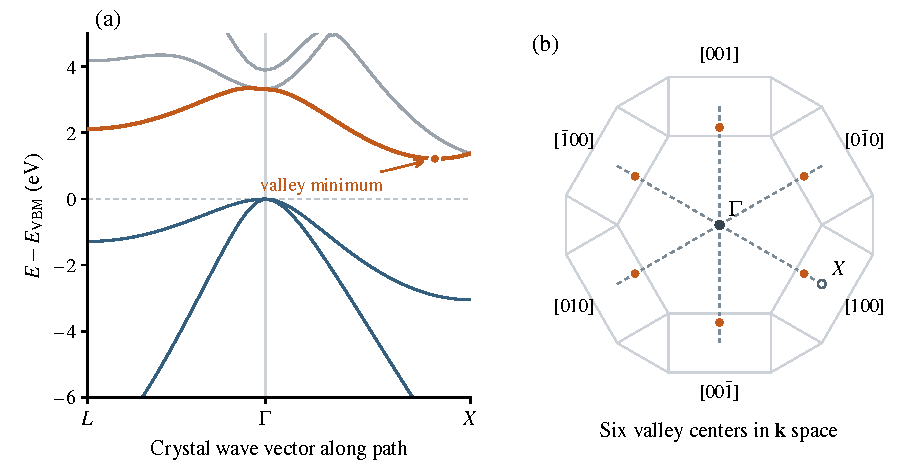
\includegraphics[width=\textwidth]{figures/silicon-band-valleys.pdf}
  \caption{Silicon bands and valleys.
  (a) HSE06 band energies for bulk diamond silicon, replotted from
  NIST JARVIS-DFT record JVASP-1002~\cite{JARVISSiHSE2026}.
  The valence-band maximum is the energy zero. Blue curves show
  valence bands; the lowest conduction band is orange and higher
  conduction bands are gray. The dot marks the sampled minimum
  between $\Gamma$ and $X$.
  (b) Positions of the six symmetry-equivalent valley centers
  (orange dots) in crystal wave-vector space. The wireframe outlines
  the first Brillouin zone; dashed lines point along the six crystal
  directions. This panel shows positions, not energy surfaces.}
  \label{fig:silicon-band-valleys}
\end{figure}
\FloatBarrier

First consider states near one minimum, at $\mathbf k_0$.
The dispersion is approximately quadratic there, so its curvature
defines an inverse effective-mass tensor
(Appendix~\ref{app:effective-mass}):
\begin{equation}
  (\mathbf M^{-1})_{\alpha\beta}
      =\frac{1}{\hbar^2}
        \left.\frac{\partial^2E_{\mathrm c}}
                     {\partial k_\alpha\partial k_\beta}
        \right|_{\mathbf k_0},
  \qquad \alpha,\beta=x,y,z.
  \label{eq:dot-band-curvature}
\end{equation}
Here $\mathbf M$ is the effective-mass tensor of the chosen valley;
it is constant in this uniform-crystal model. Its components are
written in the device coordinates $x,y,z$ defined above and need
not form a diagonal matrix.\footnote{The principal axes are the
eigenvector directions of $\mathbf M$ and need not coincide with the
device axes. Isotropy is the special case $\mathbf M=m^*\mathbf I$,
where $\mathbf I$ is the three-dimensional identity matrix.}

For confinement that varies slowly on the scale of a crystal unit
cell, we can separate the rapid spatial variation of the crystal
state from the variation across the dot. To leading order, the
spatial wave function of a confined electron has the form
\[
  \psi_n(\mathbf r)\simeq
       \chi_{\mathrm c}(\mathbf r)\phi_n(\mathbf r).
\]
Here $\chi_{\mathrm c}$ is the extended crystal state at the chosen
band minimum, while $\phi_n$ is a slowly varying, localized
\emph{envelope}; the index $n$ labels the dot orbitals. The envelope
sets the extent and shape of the electron's probability distribution
across the dot, retaining the crystal structure in $\chi_{\mathrm c}$.

Within this valley, for energies near the minimum and weak
admixture of other bands, the effective-mass reduction derived in
Appendix~\ref{app:effective-mass} gives the envelope equation
\begin{equation}
  \underbrace{
    \left[-\frac{\hbar^2}{2}\sum_{\alpha,\beta}
             (\mathbf M^{-1})_{\alpha\beta}
             \partial_{r_\alpha}\partial_{r_\beta}
          +V_{\mathrm{conf}}(\mathbf r)\right]
  }_{h_0}\phi_n=\epsilon_n\phi_n.
  \label{eq:dot-orbital-eigenproblem}
\end{equation}
Thus the orbital problem is a three-dimensional Schr\"odinger
equation with the effective-mass tensor and the device potential. The energy
of the reference crystal minimum is chosen as the zero; material
offsets and voltage shifts remain in $V_{\mathrm{conf}}$. We will use
the same reference for the dot and reservoir energies. The lowest
solution $\phi_0$ has energy $\epsilon_0$, and higher solutions describe
excited orbitals such as the level $\epsilon_1$ in
Fig.~\ref{fig:platform-device-section}(b).
Their spacing is set by confinement; for example, reducing the size
of a well increases the kinetic energy required for spatial variation
and typically increases the orbital gaps. Weak tunneling to the
reservoir allows us to treat these localized levels as states of
the dot.

The silicon--oxide or silicon--germanium interfaces that provide
vertical confinement also affect the valley states. Their potential
varies on the atomic scale and can couple crystal components near
different band minima~\cite{Friesen2010}. Thus the single-valley
orbital equation supplies one part of the electron's spatial
description. To determine the low-energy states, we must include
the interface coupling between the retained valleys.

For $N_v$ retained valleys, collect the spatial envelopes into
$\mathbf F=(F_1,\ldots,F_{N_v})^{\mathsf T}$.
The multivalley model in Appendix~\ref{app:valley-states} gives
the block Hamiltonian acting on these components:
\begin{equation}
 h_{\mathrm{mv}}=
 \begin{pmatrix}
  h_{0,1} & \hat v_{12} & \cdots & \hat v_{1,N_v}\\
  \hat v_{21} & h_{0,2} & \cdots & \hat v_{2,N_v}\\
  \vdots & \vdots & \ddots & \vdots\\
  \hat v_{N_v,1} & \hat v_{N_v,2} & \cdots & h_{0,N_v}
 \end{pmatrix}.
 \label{eq:dot-coupled-valley-equations}
\end{equation}
Each diagonal block $h_{0,\nu}$ is the orbital Hamiltonian
of Eq.~\eqref{eq:dot-orbital-eigenproblem} for valley $\nu$,
with its own effective-mass tensor and confining potential.
The off-diagonal block $\hat v_{\nu\nu'}$ transfers amplitude
from valley $\nu'$ to valley $\nu$, with
$\hat v_{\nu'\nu}=\hat v_{\nu\nu'}^\dagger$.
In the local model used here, it multiplies the spatial envelope
by a coupling function $v_{\nu\nu'}(\mathbf r)$. These functions
encode the microscopic interface structure and are additional
inputs to the effective model. The eigenstates of
$h_{\mathrm{mv}}$ are combined orbital--valley states; we denote
the lowest one by $\ket{\chi_0}$.

The consequence is particularly simple when the two lowest valleys
are equivalent and share a ground orbital $\phi_0$ of energy
$\epsilon_0$. Assume that all other orbital--valley states lie
higher in energy and that coupling to them is small compared with
their separation from this pair. Projection onto this orbital gives the valley
Hamiltonian (Appendix~\ref{app:valley-states})
\begin{equation}
 H_{\mathrm v}=\epsilon_0 I+
   \begin{pmatrix}0&v_0\\v_0^*&0\end{pmatrix}
 \quad\text{in the basis }(\ket{\nu_1},\ket{\nu_2}),
 \label{eq:dot-valley-doublet}
\end{equation}
where $v_0$ is the interface coupling matrix element within
$\phi_0$. For $v_0=|v_0|e^{i\theta_{\mathrm v}}\ne0$, the
eigenstates, energies, and valley gap are
\begin{equation}
 \begin{aligned}
  \ket{v_\pm}
    &=\frac{\ket{\nu_1}\pm e^{-i\theta_{\mathrm v}}\ket{\nu_2}}
            {\sqrt2},
  &\epsilon_\pm&=\epsilon_0\pm|v_0|,\\
  \Delta_{\mathrm{val}}&=\epsilon_+-\epsilon_-=2|v_0|.
 \end{aligned}
 \label{eq:dot-valley-eigenstates}
\end{equation}
In this limit, the lowest spatial state is
$\ket{\chi_0}=\ket{\phi_0}\otimes\ket{v_-}$. The coupling
can be small compared with an orbital excitation energy while
still determining the valley eigenstates and their entire splitting.
If mixing with excited orbitals is appreciable, the full
Hamiltonian~\eqref{eq:dot-coupled-valley-equations} determines
$\ket{\chi_0}$ and the excitation gaps without assuming this
product form.

Each spatial state also carries the electron's spin. When a common
orbital basis can be used for the retained valleys and spin-dependent
mixing is weak, we can organize the one-electron states as
\begin{equation}
  \Hilb_{N=1}\simeq
  \Hilb_{\mathrm{orb}}\otimes
  \Hilb_{\mathrm{val}}\otimes
  \mathbb{C}^{2}_{\mathrm{spin}}.
  \label{eq:single-electron-space}
\end{equation}
The first factor describes orbital envelopes, the second the
retained valley components, and the third the spin. The coupled
eigenstates need not factor into these parts. To use a single
electron as a spin qubit, we retain the lowest combined spatial
state $\ket{\chi_0}$ and use its two spin states.
Section~\ref{sec:platform-encoding} gives the conditions under
which thermal excitation and control pulses leave the electron
in that spatial state.

\subsection{When the dot contains several electrons}

Several electrons in the same well share the available one-electron
states and repel one another. Their allowed states must also satisfy
fermionic antisymmetry. The energy of an $N$-electron dot therefore
depends both on its one-electron spectrum and on the interaction
between each pair of electrons.

Let $h_1$ be the one-electron Hamiltonian acting on the orbital, valley,
and spin states retained in the description, including any relevant
valley mixing and spin-dependent energies. With spin-dependent
terms omitted, $h_1=h_{\mathrm{mv}}\otimes I_{\mathrm{spin}}$,
where $h_{\mathrm{mv}}$ is the coupled Hamiltonian in
Eq.~\eqref{eq:dot-coupled-valley-equations} and
$I_{\mathrm{spin}}$ is the identity on the two spin states.
The pair interaction $W(\mathbf r,\mathbf r')$ includes the dielectric
and conductor response to the electron charges
(Appendix~\ref{app:screened-interaction}). For $N$ electrons, this
screened repulsion gives the many-electron Hamiltonian
\begin{equation}
  H_N=\sum_{a=1}^{N}h_1^{(a)}
       +\sum_{a<b}W(\mathbf r_a,\mathbf r_b),
  \label{eq:dot-interacting-hamiltonian}
\end{equation}
where $h_1^{(a)}$ acts on electron $a$, and the second sum counts
each interacting pair once.

At fixed gate voltages and other external fields, let $E_N$ denote
the ground-state energy of $H_N$ in the antisymmetric $N$-electron
state space. The resulting sequence $E_0,E_1,E_2,\ldots$
describes the lowest energy available at each electron number.
Which number is actually occupied depends on the energy gained or
lost when electrons are exchanged with the reservoir. That comparison
is developed in Section~\ref{sec:electron-number-control}.

\subsection{Several coupled quantum dots}
\label{sec:multiple-quantum-dots}

Gate electrodes can create several potential minima, each surrounded
by barriers, in the same silicon region. We label the resulting
dots by $i$. Orthonormal localized orbitals provide a basis for specifying how
many electrons occupy each dot; several orbital--valley states and
their spin states can be retained on each dot. The barriers control
electron tunneling between dots, while Coulomb interactions act
both within and between them.

For an array isolated from reservoirs, fix the total electron number
$N$, and write $N_i$ for the number on dot $i$, so that
$N_1+N_2+\cdots=N$. The occupation tuple
$\mathbf N=(N_1,N_2,\ldots)$ defines the subspace
$\Hilb_{(N_1,N_2,\ldots)}$. The single index in $\Hilb_N$
fixes only the total number, while the tuple specifies the number
on every dot. For example, the two-electron space $\Hilb_2$ of
two dots splits into $\Hilb_{(1,1)}$, $\Hilb_{(2,0)}$, and
$\Hilb_{(0,2)}$. Each subspace contains the allowed orbital,
valley, and spin states at those occupations. In this local basis,
grouping the many-electron Hamiltonian by charge configuration
(Appendix~\ref{sec:device-orbital-basis}) gives
\begin{equation}
 \begin{aligned}
  \Hilb_N&=\bigoplus_{N_1+N_2+\cdots=N}
                 \Hilb_{(N_1,N_2,\ldots)},\\
  H_N^{(0)}&=\bigoplus_{N_1+N_2+\cdots=N}
                 H_{(N_1,N_2,\ldots)},
  \qquad H_N=H_N^{(0)}+\mathcal T.
 \end{aligned}
 \label{eq:dot-charge-blocks}
\end{equation}
Both direct sums run over the allowed occupation tuples with total
$N$. Each block $H_{(N_1,N_2,\ldots)}$ acts within the subspace with
that same tuple, and $\mathcal T$ transfers charge between different
subspaces. The superscript $(0)$ denotes the reference with these
transfers omitted. Each block then has its own ground energy
$E_{\mathbf N,0}$ and excited energies $E_{\mathbf N,a}$; the first
energy index labels the occupation tuple, and $a$ labels a level
within that subspace. These energies include the interactions
between electrons on different dots. Thus even when tunneling is
suppressed, the array need not behave as independent dots.

Restoring tunneling couples states in different charge subspaces
while preserving $N$. For two such states with uncoupled energies
$E_{\mathbf N,a}$ and $E_{\mathbf N',b}$, mixing is small when their
coupling matrix element is much smaller than
$|E_{\mathbf N,a}-E_{\mathbf N',b}|$. This is the regime used to keep
local occupations nearly fixed when the relevant charge-transfer
channels are weakly mixed. Near a degeneracy, even a small
nonzero tunnel matrix element can strongly mix the two states.
In a general orbital model, interaction terms can also transfer
charge; they belong to $\mathcal T$ along with single-electron
hopping, as detailed in Appendix~\ref{sec:device-orbital-basis}.

For a simple example, take one electron in two dots. Retain only
the lowest localized spatial state on each dot and a common fixed
spin state, assuming that coupling to other orbital--valley and spin
states can be neglected. Denote the retained states by
$\ket{1,0}$ and $\ket{0,1}$. The local-basis matrix elements in
Appendix~\ref{sec:device-orbital-basis} give
\begin{equation}
 h_{\mathrm{pair}}=
 \begin{pmatrix}
  \epsilon_1&-t_{12}\\
  -t_{12}^*&\epsilon_2
 \end{pmatrix}
 \quad\text{in the basis }(\ket{1,0},\ket{0,1}).
 \label{eq:dot-pair-hamiltonian}
\end{equation}
The diagonal entries are the energies of the two localized states,
and $t_{12}$ is their tunnel coupling, with units of energy. Gate
voltages tune both the detuning $\epsilon_1-\epsilon_2$ and the
barrier that controls $t_{12}$.
When $|\epsilon_1-\epsilon_2|\gg|t_{12}|$, each eigenstate lies
mostly in one charge subspace. When the detuning becomes comparable
to or smaller than $|t_{12}|$, both occupations contribute
appreciably. At $\epsilon_1=\epsilon_2$ and $t_{12}\ne0$, the two
eigenstates have equal weights in $(1,0)$ and $(0,1)$, with energy
separation $2|t_{12}|$ (Appendix~\ref{sec:device-orbital-basis}).
Small tunneling can therefore coexist with strong mixing near
resonance; its magnitude still sets the small splitting and the
associated slow coherent transfer.

\section{Controlling the electron number}
\label{sec:electron-number-control}

To use confined electrons as spin qubits, we must prepare the charge
configuration assumed by the spin model and retain it during control.
The single-spin qubit considered below requires one electron in a dot;
our two-dot spin model starts with one electron in each dot. A reservoir
supplies these electrons through tunneling. Gate voltages change the
dot energies to select the desired occupations, while the barriers
control how readily electrons can enter or leave. Preparing a useful
spin system therefore requires control of both its energetically
preferred electron number and its exchange of electrons with the reservoir.

To compare different electron numbers, we account for the energy of
both the dot and the reservoir that supplies its electrons. Adding
an electron to an $(N-1)$-electron dot costs $E_N-E_{N-1}$.
At zero temperature, the large reservoir loses one electron, changing
its energy by $-\mu_{\mathrm R}$, where $\mu_{\mathrm R}$ is its chemical potential.
The transfer lowers the combined energy when
$E_N-E_{N-1}-\mu_{\mathrm R}<0$. For $N$ electrons transferred
from the reservoir into the dot, the corresponding energy to compare
is $E_N-\mu_{\mathrm R}N$, up to a common reservoir reference.

We collect these charge sectors in the full dot Hamiltonian $H$,
which acts as $H_N$ in each $N$-electron sector.
At zero temperature, a dot in equilibrium with a weakly coupled
reservoir of chemical potential $\mu_{\mathrm R}$ occupies a
ground state of
\begin{equation}
  \widehat{\Omega}=H-\mu_{\mathrm R}\widehat N,
  \label{eq:dot-grand-canonical-hamiltonian}
\end{equation}
where $\widehat N$ counts electrons. In the $N$-electron sector,
this operator is $H_N-\mu_{\mathrm R}N$, whose ground-state
energy is $E_N-\mu_{\mathrm R}N$.
The equilibrium electron number is therefore
\begin{equation}
  \boxed{
  N_{\mathrm{eq}}(\mu_{\mathrm R})
    \in\operatorname*{arg\,min}_{N=0,1,\ldots}
                         [E_N-\mu_{\mathrm R}N]}.
  \label{eq:dot-equilibrium-electron-number}
\end{equation}
This determines the relation between chemical potential and
electron number from the energies $E_N$, at fixed dot parameters~\cite{Beenakker1991}.

\paragraph{Addition thresholds and charge gaps.}
Equating $E_N-\mu_{\mathrm R}N$ and
$E_{N-1}-\mu_{\mathrm R}(N-1)$ gives the threshold for adding
the $N$th electron:
\begin{equation}
  \mu_N=E_N-E_{N-1}.
  \label{eq:dot-addition-threshold}
\end{equation}
The spacing between successive thresholds is
\begin{equation}
  E_{\mathrm{add}}(N)=\mu_{N+1}-\mu_N
       =E_{N+1}-2E_N+E_{N-1}.
  \label{eq:dot-addition-energy-spacing}
\end{equation}
If $E_N$ is strictly convex, meaning $E_{\mathrm{add}}(N)>0$
for every $N\geq1$, these thresholds increase in order.
Minimizing $E_N-\mu_{\mathrm R}N$ then selects charge $N\geq1$
throughout the interval
\begin{equation}
  \mu_N<\mu_{\mathrm R}<\mu_{N+1}.
  \label{eq:dot-charge-stability-window}
\end{equation}
Each plateau has width $E_{\mathrm{add}}(N)$, so electrons enter
one at a time as $\mu_{\mathrm R}$ increases. At a boundary,
neighboring charges are degenerate; the empty dot is selected
for $\mu_{\mathrm R}<\mu_1$. Without strict convexity, some
plateaus can disappear, and the original minimization remains
the general rule.

Within a plateau, adding or removing one electron changes
the energy of $\widehat{\Omega}$ by
\begin{align}
  \Delta_+&=E_{N+1}-E_N-\mu_{\mathrm R}
             =\mu_{N+1}-\mu_{\mathrm R},\\
  \Delta_-&=E_{N-1}-E_N+\mu_{\mathrm R}
             =\mu_{\mathrm R}-\mu_N.
  \label{eq:dot-charge-transfer-costs}
\end{align}
Both costs are positive, suppressing low-energy sequential
charge transfer: this is the Coulomb-blockade regime~\cite{Beenakker1991}.

\paragraph{Selecting a charge state with gate voltages.}
Gate voltages control the electron number through their effect on
the electric potential $\Phi(\mathbf r)$ in the dot. For an electron
of charge $-e$, a potential change $\delta\Phi(\mathbf r)$ gives a
potential energy shift $-e\,\delta\Phi(\mathbf r)$. This alters the many-electron energies
$E_N$ and the addition thresholds $\mu_N=E_N-E_{N-1}$.
For a uniform shift $\delta\Phi$ over the dot,
$\delta E_N=-Ne\,\delta\Phi$, so $\delta\mu_N=-e\,\delta\Phi$.
With the reservoir chemical potential $\mu_{\mathrm R}$ held fixed,
moving a threshold across it changes the equilibrium electron
number according to Eq.~\eqref{eq:dot-equilibrium-electron-number}.
Electrical transport or charge sensing can detect this change
(Appendix~\ref{app:charge-detection}). For a given gate geometry,
a first-order expansion about a reference voltage setting
$\mathbf V_0$ relates the threshold shift to the applied voltage changes:
\begin{equation}
 \delta\mu_N\simeq-e\sum_g\alpha_{Ng}\,\delta V_g,
 \qquad
 \alpha_{Ng}=-\frac1e
       \left.\frac{\partial\mu_N}{\partial V_g}\right|_{\mathbf V_0}.
 \label{eq:platform-gate-response}
\end{equation}
Here $\alpha_{Ng}$ is the dimensionless \emph{lever arm} of gate $g$
for the $N$th addition threshold: $e\alpha_{Ng}$ converts a change
in gate voltage into a shift of that threshold. A physical gate
generally alters both the dot levels and the tunneling barriers,
so both effects must be considered when choosing the operating
voltages. Appendix~\ref{app:voltage-response} derives the corresponding
voltage responses.

\subsection{Loading a single dot}
\label{sec:single-dot-loading}

For the single-spin qubit, the two logical states are spin states
of the same confined electron. The required charge state is therefore
$N=1$. \emph{Loading} prepares this occupation by bringing an electron
from the reservoir into the dot through tunneling.

Figure~\ref{fig:single-dot-loading} shows the charge regions along
a gate-voltage scan at fixed $\mu_{\mathrm R}$. To prepare $N=1$,
first empty the dot at a setting such as $E$:
set $\mu_1-\mu_{\mathrm R}\gg k_BT$ while allowing tunneling to the reservoir,
so that an electron already in the dot can escape. Then change the
gate voltage to a setting such as $L$, where
$\mu_1<\mu_{\mathrm R}<\mu_2$, keeping the reservoir barrier low
enough to permit tunneling. An electron from an occupied reservoir
state can now enter the dot. Once it has entered, adding a second
electron costs $\mu_2-\mu_{\mathrm R}>0$, and removing the first
costs $\mu_{\mathrm R}-\mu_1>0$. Choosing both costs large compared
with $k_BT$ suppresses these further charge changes and selects
single occupation.

\begin{figure}[htbp]
 \centering
 % Single-dot charge regions as a function of gate voltage.
% Increasing V_g lowers the addition energies (positive lever arm).
% E and L denote the empty and loading operating points; the arrow is
% only the gate-voltage pulse, not a change in the tunnel barrier.
\begingroup
\definecolor{loadingGate}{HTML}{0072B2}
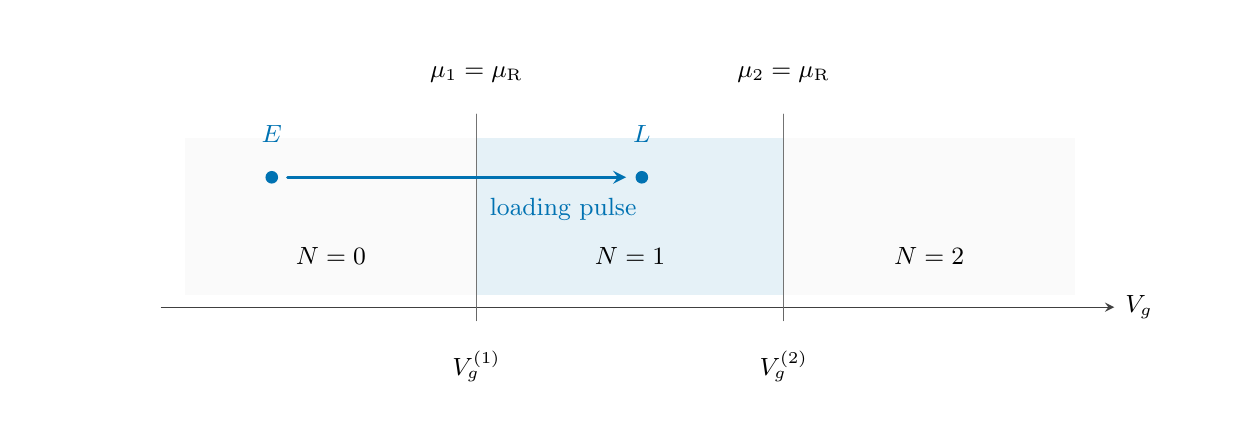
\begin{tikzpicture}[
 x=1mm,y=1mm,>=stealth,line cap=round,line join=round,
 every node/.style={font=\small,inner sep=1pt}
]
 \path[use as bounding box] (0,3) rectangle (150,52);

 % Charge sectors at a fixed reservoir chemical potential.
 \fill[black!2] (20,18) rectangle (133,38);
 \fill[loadingGate!10] (57,18) rectangle (96,38);
 \draw[black!55,line width=0.5pt] (57,16.5)--(57,41);
 \draw[black!55,line width=0.5pt] (96,16.5)--(96,41);
 \node at (38.5,23) {$N=0$};
 \node at (76.5,23) {$N=1$};
 \node at (114.5,23) {$N=2$};
 \node at (57,46) {$\mu_1=\mu_{\mathrm R}$};
 \node at (96,46) {$\mu_2=\mu_{\mathrm R}$};

 % A pulse crosses the first threshold and stops inside the N=1 interval.
 \fill[loadingGate] (31,33) circle (0.8);
 \fill[loadingGate] (78,33) circle (0.8);
 \draw[->,loadingGate,line width=1.05pt] (33,33)--(76,33);
 \node[text=loadingGate] at (31,38.5) {$E$};
 \node[text=loadingGate] at (78,38.5) {$L$};
 \node[text=loadingGate,fill=loadingGate!10,inner sep=0.5pt]
      at (68,29) {loading pulse};

 % Gate axis and charge-degeneracy voltages.
 \draw[->,black!75,line width=0.5pt] (17,16.5)--(138,16.5);
 \node[anchor=west] at (139,16.5) {$V_g$};
 \foreach \tickX in {57,96}{
  \draw[black!60,line width=0.4pt]
       (\tickX,16.5)--(\tickX,14.8);
 }
 \node at (57,9) {$V_g^{(1)}$};
 \node at (96,9) {$V_g^{(2)}$};
\end{tikzpicture}
\endgroup

 \caption{Single-dot charge regions at fixed reservoir chemical
 potential $\mu_{\mathrm R}$. For the gate response illustrated here,
 increasing $V_g$ lowers the addition thresholds. The voltages
 $V_g^{(1)}$ and $V_g^{(2)}$ satisfy $\mu_1=\mu_{\mathrm R}$ and
 $\mu_2=\mu_{\mathrm R}$, respectively. The loading pulse moves from
 the empty-dot setting $E$ into the $N=1$ region at $L$, while
 tunneling to the reservoir remains possible. Raising the reservoir
 barrier after loading is a separate step.}
 \label{fig:single-dot-loading}
\end{figure}

Crossing the addition threshold makes entry energetically favorable;
the dot still has to wait for an electron to tunnel through the
barrier. The loading voltages are therefore held for a finite
interval, long compared with the typical entry waiting time, which
depends on the barrier transparency. After this loading interval,
raising the reservoir barrier reduces electron exchange and retains
the electron while its spin is manipulated. For an unwanted escape
rate $\Gamma_{\mathrm{escape}}$ and a control interval $\tau$, the
condition $\Gamma_{\mathrm{escape}}\tau\ll1$ makes loss during that
interval unlikely. Energetic stability suppresses unwanted charge
changes through their energy costs; a high barrier additionally
suppresses the tunneling that would carry them out.

\FloatBarrier
\subsection{Loading two coupled dots}
\label{sec:double-dot-loading}

The two-dot spin model used below requires one localized spin on
each dot. Its starting charge configuration is therefore $(N_1,N_2)=(1,1)$.
Preparing it requires selecting the occupation of each dot, since
two electrons in the pair could also occupy $(2,0)$ or $(0,2)$.

The plunger-gate voltages $V_1,V_2$ tune the dot energies. Repulsion
between dots makes each addition threshold depend on the occupation
of the other dot. With the reservoirs at a common chemical potential
$\mu_{\mathrm R}$ and interdot mixing neglected, the equilibrium
condition partitions the $(V_1,V_2)$ plane into regions of fixed
$(N_1,N_2)$ (Appendix~\ref{app:charge-stability}).
Figure~\ref{fig:measurement-honeycomb} shows the resulting
\emph{charge stability diagram} around $(1,1)$. Crossing a blue
boundary exchanges an electron with a reservoir; for example,
$(1,0)\to(1,1)$ loads dot 2. Crossing an orange boundary transfers
an electron between dots while preserving their total number;
for example, $(1,1)\to(2,0)$ moves an electron from dot 2 to dot 1.

\begin{figure}[htbp]
 \centering
 % A local honeycomb neighborhood with the usual negatively sloping
% reservoir transitions and positively sloping interdot transitions.
\begingroup
\small
\setlength{\unitlength}{1mm}
\begin{picture}(150,87)
 \put(15,8){\vector(1,0){122}}
 \put(15,8){\vector(0,1){73}}
 \put(137,4){\makebox(10,7){$V_1$}}
 \put(5,78){\makebox(10,7){$V_2$}}
 \put(66,35){\makebox(25,8){$(1,1)$}}
 \put(32,26){\makebox(25,8){$(0,1)$}}
 \put(53,11){\makebox(25,8){$(1,0)$}}
 \put(90,18){\makebox(25,8){$(2,0)$}}
 \put(106,44){\makebox(25,8){$(2,1)$}}
 \put(83,62){\makebox(25,8){$(1,2)$}}
 \put(28,62){\makebox(25,8){$(0,2)$}}
 \linethickness{0.9pt}
 \color{blue!65!black}
 % Central cell A(51,29), B(83,21), C(103,37),
 % D(95,61), E(63,69), F(43,53).
 \qbezier(51,29)(67,25)(83,21)
 \qbezier(103,37)(99,49)(95,61)
 \qbezier(95,61)(79,65)(63,69)
 \qbezier(43,53)(47,41)(51,29)
 % Reservoir-transition edges extending to adjacent cells.
 \qbezier(83,21)(85,15)(87,9)
 \qbezier(103,37)(118,33.25)(133,29.5)
 \qbezier(63,69)(61,75)(59,81)
 \qbezier(43,53)(31.5,55.875)(20,58.75)
 \color{orange!85!black}
 \qbezier(83,21)(93,29)(103,37)
 \qbezier(63,69)(53,61)(43,53)
 \qbezier(51,29)(40,20.2)(29,11.4)
 \qbezier(95,61)(107,70.6)(119,80.2)
 \color{black}
 \put(51,29){\circle*{2}}
 \put(83,21){\circle*{2}}
 \put(103,37){\circle*{2}}
 \put(95,61){\circle*{2}}
 \put(63,69){\circle*{2}}
 \put(43,53){\circle*{2}}
\end{picture}
\endgroup

 \caption{Schematic charge regions of two dots with negligible
 interdot mixing and a common reservoir chemical potential.
 Blue boundaries change the total electron number by one;
 orange boundaries transfer an electron between dots.
 Black points, called triple points, mark where three charge regions
 meet. The central $(1,1)$ region provides the charge configuration
 for one localized spin on each dot. The axes are plunger voltages;
 offsets, scales, and cross-couplings are unspecified.}
 \label{fig:measurement-honeycomb}
\end{figure}

To prepare $(1,1)$, choose voltages inside its region, sufficiently
far from the boundaries that unwanted charge changes cost much more
than $k_BT$. Allow exchange with the reservoirs long enough for the
occupations to equilibrate, then raise the reservoir barriers to
retain the two electrons. The interdot tunnel coupling must also
remain small compared with the relevant charge-transfer gaps to
keep the occupations close to one electron per dot. Appendix~\ref{app:charge-stability}
derives the boundary conditions and explains how measured charge
transitions locate these regions.

\FloatBarrier
\section{Qubit architectures and encodings}
\label{sec:qubit-architectures}

After selecting and retaining the $N=1$ charge state, we can keep
the electron in the lowest orbital--valley state $\ket{\chi_0}$ and
use its two spin states to store a qubit. With several confined
electrons, we can instead select two joint spin states and use them
as one logical qubit. The choice of this two-dimensional
\emph{computational subspace} is the encoding; transitions out of
it are leakage. Different encodings use the available physical
interactions differently: a field acts on an individual spin,
while an interaction between spins can act within a jointly
encoded space.

We retain one orbital--valley state per dot and assume predominantly
one electron per occupied dot.

\subsection{Single-spin qubits}
\label{sec:single-spin-qubits}

For one electron, we choose the logical basis
\begin{equation}
  \ket{0}=\ket{\chi_0}\otimes\ket{\downarrow},
  \qquad
  \ket{1}=\ket{\chi_0}\otimes\ket{\uparrow}.
  \label{eq:qubit-basis}
\end{equation}
The computational space is
$\Hilb_{\mathrm q}=\operatorname{span}\{\ket0,\ket1\}$,
and a pure qubit state is $\ket{\psi}=a\ket0+b\ket1$, with
$|a|^2+|b|^2=1$.
Leakage involves charge, orbital, or valley excitations.

Charge preparation alone does not fix the spin state.
For example, the two-dot $(1,1)$ charge configuration introduced
in Section~\ref{sec:multiple-quantum-dots}, with one orbital--valley
state per dot, contains four spin states:
\begin{equation}
  \ket{\downarrow\downarrow},\quad
  \ket{\downarrow\uparrow},\quad
  \ket{\uparrow\downarrow},\quad
  \ket{\uparrow\uparrow}.
  \label{eq:two-spin-basis}
\end{equation}
The arrows refer to dots 1 and 2. A charge stability diagram identifies
charge occupations and transitions, not the spin state within a charge
sector; its boundaries are derived in
Appendix~\ref{sec:measurement-double-dot-csd}.
The four states can represent two single-spin qubits or supply
a subspace for one encoded qubit~\cite{Burkard2023}.

\subsection{Singlet--triplet qubits}
\label{sec:singlet-triplet-qubits}

Two spins decompose as $\tfrac12\otimes\tfrac12=0\oplus1$.
We encode one qubit in the $m=0$ states: the singlet ($S=0$) and
the triplet ($S=1$),\footnote{The label $S$ in $\ket S$ stands for
``singlet''; the total-spin quantum number of this state is $S=0$.}
\begin{equation}
  \begin{aligned}
    \ket{0_{\mathrm{ST}}}=\ket{S}
      &=\frac{\ket{\uparrow\downarrow}-\ket{\downarrow\uparrow}}{\sqrt{2}},\\
    \ket{1_{\mathrm{ST}}}=\ket{T_0}
      &=\frac{\ket{\uparrow\downarrow}+\ket{\downarrow\uparrow}}{\sqrt{2}}.
  \end{aligned}
  \label{eq:st-basis}
\end{equation}
The remaining triplets
$\ket{T_+}=\ket{\uparrow\uparrow}$ and
$\ket{T_-}=\ket{\downarrow\downarrow}$ are spin-leakage states.

\subsection{Exchange-only qubits}
\label{sec:exchange-only-qubits}

Three spin-$1/2$ electrons can encode one logical qubit. Their spin
space decomposes as
\[
 \tfrac12\otimes\tfrac12\otimes\tfrac12
   =\tfrac12\oplus\tfrac12\oplus\tfrac32.
\]
Taking the $m=+1/2$ state from each of the two $S=1/2$
representations gives a two-dimensional computational space.
We choose the basis
\begin{equation}
  \begin{aligned}
    \ket{0_{\mathrm E}}&=
       \frac{\ket{\uparrow\downarrow\uparrow}
             -\ket{\downarrow\uparrow\uparrow}}{\sqrt{2}},\\
    \ket{1_{\mathrm E}}&=
       \frac{2\ket{\uparrow\uparrow\downarrow}
             -\ket{\uparrow\downarrow\uparrow}
             -\ket{\downarrow\uparrow\uparrow}}{\sqrt{6}}.
  \end{aligned}
  \label{eq:exchange-only-basis}
\end{equation}
The arrows refer to spins 1, 2, and 3.
Spins 1 and 2 form a singlet in $\ket{0_{\mathrm E}}$ and a triplet
in $\ket{1_{\mathrm E}}$, distinguishing the two $S=1/2$ representations.
The spin-rotation-invariant interaction derived in
Section~\ref{sec:exchange-virtual-tunneling} is called isotropic exchange.
It preserves $S,m$ but can mix these two states, allowing logical
rotations using exchange alone (Section~\ref{sec:encoded-gates}).

\section{Engineering spin control and exchange interactions}
\label{sec:spin-control-exchange}

An encoding specifies which states store quantum information.
To manipulate that information, we need a Hamiltonian that changes
relative phases or populations within the chosen spin space.
A static magnetic field splits the two levels of an individual
spin and makes their relative phase evolve. A transverse drive
mixes those levels, while tunneling between dots produces an
exchange interaction that couples different spins. These physical
terms supply the controls whose action on each encoding is worked
out in Section~\ref{sec:quantum-gates}.

The spin description assumes that charge, orbital, and valley
excitations can be excluded as independent computational states.
This restriction must remain valid at the operating field and
under the applied pulses, even when virtual excitations contribute
to the effective spin Hamiltonian~\cite{Burkard2023}.

\subsection{Zeeman splitting and the two-level approximation}
\label{sec:platform-encoding}

Consider a singly occupied dot with the electron in the spatial
state $\ket{\chi_0}$. A static magnetic field along $+z$ lifts the
degeneracy of its two spin states. For a positive isotropic
effective $g$ factor, the Zeeman Hamiltonian in the physical-spin
basis $(\ket{\uparrow},\ket{\downarrow})$ is
\begin{equation}
  H_Z=\frac{E_Z}{2}\sigma_z,
  \qquad E_Z=g\mu_B B>0.
  \label{eq:zeeman}
\end{equation}
Here $\mu_B$ is the Bohr magneton and $B$ the field magnitude.
With the logical basis in Eq.~\eqref{eq:qubit-basis},
$\ket0$ is the lower level and $\ket1$ the upper level.
In this basis, $H_Z|_{\Hilb_{\mathrm q}}=-E_ZZ/2$.
The minus sign follows from assigning the lower spin level to
$\ket0$. This diagonal Hamiltonian changes the relative phase of
a spin superposition while leaving the two populations unchanged.

The two-level approximation requires the electron to remain in the
retained orbital--valley state and charge sector. Let
$\Delta_{\mathrm{orb}}$ and $\Delta_{\mathrm{val}}$ denote the
relevant gaps to excluded orbital and valley states, measured at the
operating field (Appendix~\ref{app:dot-spectroscopy}). The condition
$k_BT\ll\min(\Delta_{\mathrm{orb}},\Delta_{\mathrm{val}})$
suppresses their thermal occupation. If electron exchange with a
reservoir remains possible, every accessible charge-transfer process
out of either retained spin state must have a positive energy cost
large compared with $k_BT$. The costs $\Delta_\pm$ in
Eq.~\eqref{eq:dot-charge-transfer-costs} refer to the ground state
of the occupied charge sector, with $E_N$ evaluated including the
Zeeman energies at the operating field. Starting in its upper Zeeman state
reduces a transfer cost by $E_Z$ for the same final state.
Alternatively, reservoir exchange can be made negligible on the
operation timescale by raising its tunnel barrier. Low temperature
alone does not prevent
control-induced leakage: a pulse that couples to an excluded state
can populate it if its frequency approaches the corresponding
transition. The coupling matrix elements, excitation gaps, and
pulse spectrum must therefore be checked together~\cite{Burkard2023}.

Both Zeeman states belong to the retained qubit space. Keeping the
electron in that space does not require it to occupy only the
lower spin level, and does not by itself require $k_BT\ll E_Z$.
That stronger spin-polarization condition is useful when thermal
relaxation is used to prepare $\ket0$. During coherent operations,
the intended state may instead be any superposition of the two
levels. Spin relaxation and loss of phase coherence constrain how
long that state can be retained even when charge, orbital, and
valley leakage remain negligible.

\subsection{Transverse spin control}
\label{sec:transverse-spin-control}

Our aim is to control both the relative phase and the populations
of the two spin states. A suitable Hamiltonian is
\begin{equation}
  H_{\mathrm{target}}(t)=a(t)\sigma_z+b(t)\sigma_x,
  \label{eq:single-spin-control-target}
\end{equation}
where $a,b$ are real energy coefficients.
The $\sigma_z$ term changes the relative phase of $\ket{\uparrow}$
and $\ket{\downarrow}$, while $\sigma_x$ mixes them.
A static Zeeman field already supplies the longitudinal term.
We need to generate a useful transverse term, either directly in
the laboratory or in an effective rotating frame.

A constant transverse coupling is the simplest candidate. To see
its limitation, keep the Zeeman splitting fixed and switch on
a term $\hbar\Omega_x\sigma_x/2$ at $t=0$:
\begin{equation}
  H_{\mathrm{static}}=\frac{\hbar}{2}
     (\omega_Z\sigma_z+\Omega_x\sigma_x),\qquad
  \omega_Z=\frac{E_Z}{\hbar}.
  \label{eq:static-transverse-hamiltonian}
\end{equation}
Since $(\omega_Z\sigma_z+\Omega_x\sigma_x)^2
=(\omega_Z^2+\Omega_x^2)I$, a spin initially in $\ket{\downarrow}$
has transition probability
\begin{equation}
  P^{\mathrm{static}}_{\downarrow\to\uparrow}(t)
   =\frac{\Omega_x^2}{\omega_Z^2+\Omega_x^2}
      \sin^2\!\left(\frac{t}{2}\sqrt{\omega_Z^2+\Omega_x^2}\right),
  \qquad
  P_{\max}^{\mathrm{static}}
   =\frac{\Omega_x^2}{\omega_Z^2+\Omega_x^2}.
  \label{eq:static-transverse-probability}
\end{equation}
For $|\Omega_x|\ll\omega_Z$, the maximum is approximately
$(\Omega_x/\omega_Z)^2\ll1$, regardless of pulse duration. The spin rotates about $(\Omega_x,0,\omega_Z)$,
an axis close to $z$, so it cannot reach the opposite Zeeman state.
With zero longitudinal splitting, a full flip would take
$\pi/|\Omega_x|$; the bound applies to a single constant pulse
with fixed $\omega_Z$.

Resonant driving avoids this limitation by making the transverse
coupling oscillate near the Zeeman frequency.

\paragraph{Resonant driving and Rabi oscillations.}
Keep the Zeeman splitting fixed and take an oscillating transverse
term with real drive coefficient $\Omega$, angular frequency
$\omega$ and phase $\phi$ (Appendix~\ref{app:transverse-drive-origins}):
\begin{equation}
  H(t)=\frac{\hbar\omega_Z}{2}\sigma_z
       +\hbar\Omega\cos(\omega t+\phi)\sigma_x,
  \qquad \omega_Z=\frac{E_Z}{\hbar}.
  \label{eq:esr-lab}
\end{equation}
The drive couples the Zeeman states because
$\bra{\uparrow}\sigma_x\ket{\downarrow}=1$.
In a frame rotating at the drive frequency,
$\ket{\psi(t)}=e^{-i\omega t\sigma_z/2}\ket{\psi_{\mathrm r}(t)}$,
define the detuning $\delta=\omega_Z-\omega$.
For $|\delta|,|\Omega|\ll\omega_Z$, the rotating-wave approximation
(RWA) gives the effective Hamiltonian and evolution
(Appendix~\ref{app:spin-driving})
\begin{equation}
  \begin{aligned}
    H_{\mathrm{RWA}}&=\frac{\hbar}{2}
      \left[\delta\sigma_z
        +\Omega(\cos\phi\,\sigma_x+\sin\phi\,\sigma_y)\right],\\
    U_{\mathrm r}(t)&=\cos\frac{\Omega_{\mathrm{eff}}t}{2}\,I
      -i\sin\frac{\Omega_{\mathrm{eff}}t}{2}\,
       \frac{\delta\sigma_z
         +\Omega(\cos\phi\,\sigma_x+\sin\phi\,\sigma_y)}
            {\Omega_{\mathrm{eff}}},
  \end{aligned}
  \label{eq:esr-propagator}
\end{equation}
where $\Omega_{\mathrm{eff}}=\sqrt{\delta^2+\Omega^2}$ is the rotation
frequency. The phase sets the transverse direction of the rotation
axis $(\Omega\cos\phi,\Omega\sin\phi,\delta)$. For $\phi=0$,
the target coefficients are $a=\hbar\delta/2$ and $b=\hbar\Omega/2$.
To find the pulse duration for a spin flip, start in
$\ket{\downarrow}$ and evaluate the up-spin probability:
\begin{equation}
  P_{\downarrow\to\uparrow}(t)
    =\frac{\Omega^2}{\delta^2+\Omega^2}
       \sin^2\!\left(\frac{t}{2}\sqrt{\delta^2+\Omega^2}\right).
  \label{eq:rabi-probability}
\end{equation}
This population-transfer probability is independent of $\phi$.
Tune the drive frequency to the measured spin resonance to set
$\delta=0$ (Appendix~\ref{sec:measurement-spin-spectroscopy}).
The measured rotation rate at the chosen drive amplitude then sets
the spin-flip duration $t_\pi=\pi/|\Omega|$, even for
$|\Omega|\ll\omega_Z$.
Detuning tilts the effective rotation axis and reduces the maximum
inversion. High-fidelity inversion therefore requires
$|\delta|\ll|\Omega|$ and a pulse shorter than the coherence time.

\subsection{Exchange from virtual tunneling}
\label{sec:exchange-virtual-tunneling}

For electron spins confined in neighboring quantum dots, tunneling
through the interdot barrier provides an exchange interaction whose
strength can be controlled electrically. Together with the single-spin
controls described above, this interaction supplies the means to
implement two-spin gates. In the regime of interest, the electron
pair remains predominantly in the $(1,1)$ configuration: double occupation is energetically
costly, but its weak admixture can still affect the spin dynamics.

\paragraph{Virtual tunneling and exchange.}
Consider a double dot isolated from its reservoirs, so that its total
electron number remains fixed at two. Tunneling connects the $(1,1)$
configuration to $(2,0)$ and $(0,2)$ by transferring an electron onto
the occupied neighboring dot. To describe these processes, we retain
one orbital--valley state on each dot, with both spin states, and
assume that tunneling conserves spin. The Hubbard approximation
developed in Appendix~\ref{sec:device-hubbard-reduction} gives
\begin{equation}
  \begin{aligned}
    H_{\mathrm{Hub}}
      &=\sum_{i=1}^2\epsilon_i n_i
        +U\sum_{i=1}^2 n_{i\uparrow}n_{i\downarrow}+Vn_1n_2\\
      &\quad-t_c\sum_{\sigma=\uparrow,\downarrow}
        (c_{1\sigma}^\dagger c_{2\sigma}
         +c_{2\sigma}^\dagger c_{1\sigma}).
  \end{aligned}
  \label{eq:two-site-hubbard}
\end{equation}
Here $c_{i\sigma}$ annihilates an electron with spin $\sigma$ on
dot $i$. The occupation operators are
$n_{i\sigma}=c_{i\sigma}^\dagger c_{i\sigma}$ and
$n_i=n_{i\uparrow}+n_{i\downarrow}$.
Each retained orbital has energy $\epsilon_i$, while the Coulomb
repulsion depends on whether the electrons occupy the same dot or
different dots. These two cases contribute the energies $U$ and $V$,
respectively; for simplicity, we take the same $U$ on both dots.
The final term transfers an electron between the dots with real
tunnel amplitude $t_c$. This model neglects direct Coulomb exchange,
and we leave out the local Zeeman terms when calculating the exchange
contribution.

The energetic cost of a tunneling process follows from both the
orbital energies and the repulsion. Moving an electron onto the
occupied dot replaces the interdot repulsion $V$ with the on-site
repulsion $U$. It also changes the orbital energy by
$+\varepsilon$ or $-\varepsilon$, depending on the direction of
transfer, where $\varepsilon=\epsilon_1-\epsilon_2$.
The two double-occupation costs, measured from the energy of $(1,1)$
in the absence of tunneling, are therefore
\begin{equation}
  \Delta_{20}=U-V+\varepsilon,\qquad
  \Delta_{02}=U-V-\varepsilon.
  \label{eq:virtual-charge-gaps}
\end{equation}
We choose an operating point at which both costs are positive and
much larger than $|t_c|$. Tunneling then mixes only small components
of the doubly occupied states into the low-energy states associated
with $(1,1)$. Provided thermal and drive-induced charge excitation
are also negligible, the doubly occupied states can be eliminated
from the low-energy description while retaining the energy shifts
that their virtual mixing produces.

The spin dependence of these shifts follows from fermionic
antisymmetry. Within the retained orbital--valley state, a doubly
occupied dot can support only a spin singlet. The $(1,1)$ singlet
can therefore mix with both higher-energy charge states, whereas
the triplets have no such tunneling channel. This mixing lowers
the singlet energy and leaves the triplet energy unchanged.
Eliminating the two charge states to second order in $t_c$ gives
the singlet--triplet energy difference
(Appendix~\ref{sec:device-low-energy-reduction})
\begin{equation}
  J\equiv E_T-E_S
     =2t_c^2\left(\frac{1}{\Delta_{20}}+\frac{1}{\Delta_{02}}\right).
  \label{eq:superexchange}
\end{equation}
This energy difference is the exchange coupling that enters the
spin Hamiltonian. After the higher-energy charge states have been
eliminated, the interaction within the $(1,1)$ spin space takes
the Heisenberg form~\cite{Loss1998}
\begin{equation}
  H_{\mathrm{ex}}=J\,\mathbf{s}_1\cdot\mathbf{s}_2.
  \label{eq:exchange-spin}
\end{equation}
A common energy shift has been omitted. The charge degrees of freedom
thus enter the spin dynamics through the coefficient $J$, whose value
is set by the tunnel amplitude and the two double-occupation costs.

\paragraph{Tuning exchange with gate voltages.}
Gate voltages control this interaction by changing the interdot
tunneling and the relative orbital energies. Substituting the charge
costs into the expression for $J$ makes these dependencies explicit:
\begin{equation}
  J(\varepsilon)=\frac{4t_c^2(U-V)}{(U-V)^2-\varepsilon^2},\qquad
  J(0)=\frac{4t_c^2}{U-V}.
  \label{eq:exchange-detuning}
\end{equation}
Adjusting the interdot barrier changes the tunnel amplitude $t_c$,
while shifting the orbital energy of one dot relative to the other
changes the detuning $\varepsilon$. The tunnel amplitude at the
chosen barrier setting must be measured
(Appendix~\ref{sec:measurement-tunnel-spectroscopy}); the exchange
strength used to set a spin pulse is calibrated at the corresponding
compensated voltages (Appendix~\ref{sec:calibration-two-spin-exchange}).
In either case, the resulting
exchange pulse must remain within the regime used to obtain the
spin Hamiltonian. If a double-occupation cost becomes comparable
to $|t_c|$, the associated charge state mixes strongly with $(1,1)$
and must be included explicitly in the dynamics. The apparent
divergence of the expression for $J$ near a charge degeneracy is
therefore outside its range of validity.

In a device, changing the barrier voltage generally changes the
tunnel amplitude and shifts the dot levels at the same time. A pulse intended to tune
exchange can consequently move the addition thresholds that define
the chosen charge operating point. These shifts can be compensated
by adjusting the two plunger voltages together with the barrier
voltage.

For a small barrier-voltage change $\delta V_{\mathrm B}$, let
$\delta\mathbf V_{\mathrm P}$ denote the two plunger adjustments
and $\delta\boldsymbol\mu$ the resulting shifts of the two addition
thresholds. The matrix $G_{\mathrm P}$ contains the measured
derivatives of these thresholds with respect to the two plunger
voltages at the operating point, while the vector $\mathbf g_{\mathrm B}$
contains their measured derivatives with respect to the barrier
voltage. With independent plunger responses,
$G_{\mathrm P}$ is invertible, and the voltage response gives the
compensation required to keep both thresholds fixed
(Appendix~\ref{app:virtual-gates}):
\begin{equation}
 \delta\boldsymbol\mu
    =G_{\mathrm P}\delta\mathbf V_{\mathrm P}
          +\mathbf g_{\mathrm B}\delta V_{\mathrm B},
 \qquad
 \left.\delta\mathbf V_{\mathrm P}\right|_{\delta\boldsymbol\mu=0}
    =-G_{\mathrm P}^{-1}\mathbf g_{\mathrm B}\delta V_{\mathrm B}.
 \label{eq:platform-compensated-voltage}
\end{equation}
Coordinated voltage combinations chosen to control specified
quantities are called \emph{virtual gates}. This combination cancels
the changes in the two chosen thresholds to first order around the
operating point, while allowing the tunnel amplitude and other
Hamiltonian parameters to vary.

\section{Initialization and spin readout}
\label{sec:initialization-readout}

Initialization prepares a known logical input; readout converts the
logical basis populations into distinguishable electrical signals.
The readout schemes considered here first convert the spin
distinction into different charge configurations or tunneling
records. A nearby charge sensor detects these through their
electric effect on its current (Appendix~\ref{sec:measurement-charge-sensor}).

\subsection{Single-spin qubits}
\label{sec:single-spin-spam}
\label{sec:spin-initialization}

The initialization target is $\ket0=\ket{\downarrow}$, and readout
distinguishes $\ket{\downarrow}$ from $\ket{\uparrow}$.
We suppress the common orbital--valley state in the notation.
The lower spin state can be prepared either by relaxation after
loading or by selecting it during loading.

\paragraph{Initialization by relaxation.}
First load one electron from a reservoir. Its spin may initially
occupy either Zeeman level. Raising the reservoir barrier then
suppresses electron exchange and keeps the dot occupied.
The spin remains coupled to the thermal environment, so an excited
$\ket{\uparrow}$ can release energy and relax to the lower
$\ket{\downarrow}$ state. Waiting for this dissipative process
prepares the input state; a unitary rotation alone cannot reset an
arbitrary unknown spin.

The achievable ground-state population and required waiting time
follow from the relaxation dynamics. Let $p_\uparrow(t)$ be the
probability of occupying the upper spin level.
For a bath at temperature $T$, its equilibrium value is
$p_\uparrow^{\mathrm{eq}}=[1+\exp(E_Z/k_BT)]^{-1}$, where $k_B$
is Boltzmann's constant. A simple relaxation model is
\begin{equation}
  \dot p_\uparrow=-\frac{p_\uparrow-p_\uparrow^{\mathrm{eq}}}{T_1},
  \qquad
  p_\uparrow(t)=p_\uparrow^{\mathrm{eq}}
       +[p_\uparrow(0)-p_\uparrow^{\mathrm{eq}}]e^{-t/T_1}.
  \label{eq:thermal-spin-initialization}
\end{equation}
Here $T_1$ is the longitudinal relaxation time.
The initial-state dependence decays on the scale $T_1$, but the
remaining excited-state population is set by the bath temperature.
High-probability ground-state preparation therefore requires both
a wait much longer than $T_1$ and $E_Z\gg k_BT$.
Use the measured $T_1$ and long-time excited-state population at the
holding voltages to choose the waiting time and determine the
attainable preparation probability
(Appendix~\ref{sec:measurement-relaxation}). The loading and isolation
settings are specified in
Appendix~\ref{sec:calibration-single-spin-initialization}.

\paragraph{Spin-selective loading.}
The second method prepares the lower spin state as the electron
enters the dot, without relying on subsequent spin relaxation.
Start from an empty dot. The energy required to add the first
electron is $\mu_\sigma=E(1,\sigma)-E(0)$, where $E(0)$ and
$E(1,\sigma)$ are the empty-dot and one-electron energies.
Its spin dependence comes from the Zeeman energy of the final state.
If $\epsilon_d$ is the addition energy without the Zeeman term,
\begin{equation}
  \mu_\downarrow=\epsilon_d-\frac{E_Z}{2},\qquad
  \mu_\uparrow=\epsilon_d+\frac{E_Z}{2}.
  \label{eq:spin-resolved-addition-energies}
\end{equation}
Thus the two loading thresholds differ by $E_Z$ even for the first
electron, without an electron--electron interaction.
Gate voltages shift their common position $\epsilon_d$ relative to
the reservoir chemical potential $\mu_{\mathrm R}$.
To allow down-spin loading while suppressing up-spin loading, set
\begin{equation}
  \mu_\downarrow<\mu_{\mathrm R}<\mu_\uparrow.
  \label{eq:spin-selective-window}
\end{equation}
The spin-resolved addition thresholds must be measured to select
the plunger voltage that satisfies this window
(Appendix~\ref{sec:calibration-single-spin-readout}).
At low temperature, reservoir states at $\mu_\downarrow$ are
occupied and can supply an electron, while states at
$\mu_\uparrow$ are mostly empty. Charging energy must also prevent
a second electron from entering.

The level alignment determines which process is allowed; the tunnel
rates determine how long to keep the loading window open.
For weak spin-conserving tunneling, let $\Gamma_\sigma$ be the bare
tunnel rate and $T_e$ the reservoir electron temperature.
The Fermi occupation factor gives the conditional rates
\begin{equation}
  \begin{aligned}
    f_{\mathrm R}(E)&=\frac{1}{1+\exp[(E-\mu_{\mathrm R})/(k_BT_e)]},\\
    \Gamma_{\mathrm{in},\sigma}&=\Gamma_\sigma f_{\mathrm R}(\mu_\sigma),
    \qquad
    \Gamma_{\mathrm{out},\sigma}
       =\Gamma_\sigma[1-f_{\mathrm R}(\mu_\sigma)].
  \end{aligned}
  \label{eq:reservoir-spin-rates}
\end{equation}
The factors $f_{\mathrm R}$ and $1-f_{\mathrm R}$ require an
occupied source state and an empty destination state, respectively.
Appendix~\ref{sec:amplitudes-to-master-equation} derives these
reservoir rates and their waiting-time law from tunneling amplitudes.
Both margins in Eq.~\eqref{eq:spin-selective-window} should exceed
$k_BT_e$ and tunnel broadening so that loading and unloading remain
spin-selective.

Neglecting other events, an initially empty dot remains empty with
probability $e^{-\Gamma_{\mathrm{in},\downarrow}t}$.
Measure the loading rate at the chosen reservoir-barrier setting
(Appendix~\ref{sec:calibration-single-spin-initialization}) and use
it to choose a loading interval much longer than
$\Gamma_{\mathrm{in},\downarrow}^{-1}$. Then raise the reservoir
barrier to retain the electron during the gate sequence.
Spin-selective loading has been demonstrated in
$\Si/\Si\Ge$ dots~\cite{Simmons2011}.
Excited orbitals and energy-dependent barriers can modify the rates.

\paragraph{Readout by energy-selective tunneling.}
\label{sec:energy-selective-readout}

The readout goal is to determine whether the occupied dot contains
an up-spin or down-spin electron after the gates.
We convert that distinction into a charge transient by allowing
only the upper spin level to empty into the reservoir.

Reopen the reservoir barrier and tune the addition energies to
Eq.~\eqref{eq:spin-selective-window}.
An up-spin electron can tunnel into an empty reservoir state;
a down-spin electron remains because the corresponding states
are occupied. If the dot empties, it can reload a down-spin electron.
The two initial spin states therefore give different charge records:
\begin{equation}
  \begin{aligned}
    \ket{\uparrow}:&\quad N=1\longrightarrow0\longrightarrow1,\\
    \ket{\downarrow}:&\quad N=1\quad\text{throughout the readout interval}.
  \end{aligned}
  \label{eq:energy-readout-records}
\end{equation}
A sensor dot or quantum point contact detects the temporary empty
state through a current or radio-frequency response~\cite{Elzerman2004}.
The evidence for an initial up spin is the $1\to0\to1$ transient,
not the final occupation, which can be one for either spin.

The electron must escape before it relaxes: a spin that relaxes first
leaves no up-spin charge record. To quantify this competition, take
constant escape and relaxation rates
$\Gamma_{\mathrm{out},\uparrow}$ and $T_1^{-1}$
during a low-temperature readout interval $\tau_{\mathrm r}$.
The probability of neither event by time $t$ is
$e^{-(\Gamma_{\mathrm{out},\uparrow}+T_1^{-1})t}$.
Multiplying by the escape rate and integrating gives the probability
of producing the desired charge transient:
\begin{equation}
  P_{\mathrm{escape}|\uparrow}(\tau_{\mathrm r})
    =\frac{\Gamma_{\mathrm{out},\uparrow}}
           {\Gamma_{\mathrm{out},\uparrow}+T_1^{-1}}
      \left[1-e^{-(\Gamma_{\mathrm{out},\uparrow}+T_1^{-1})\tau_{\mathrm r}}\right].
  \label{eq:readout-competing-rates}
\end{equation}
Even when escape occurs, the detector must resolve the empty interval.
Fast reloading or sensor noise can hide it, while thermal down-spin
escape can produce a false up-spin signal.
Thus readout fidelity depends on the charge-conversion probability
above and on the sensor response. The measured escape rates and
$T_1$ at the readout voltages determine the reservoir-barrier setting
and readout interval: up-spin escape should be likely before
relaxation, while down-spin escape remains unlikely
(Appendix~\ref{sec:calibration-readout-duration-choice}).

For $a\ket{\downarrow}+b\ket{\uparrow}$, ideal readout gives the
up-spin outcome with probability $|b|^2$. Measurements after
calibrated rotations on repeated preparations access other spin
components. Escape and reloading make this protocol destructive.
Appendix~\ref{sec:calibration-single-spin-readout} specifies the
conversion window, and Appendix~\ref{sec:calibration-readout-duration-choice}
derives the competing-rate probability and duration constraints.

\subsection{Singlet--triplet qubits}
\label{sec:st-spam}
\label{sec:pauli-blockade-readout}

Here initialization prepares $\ket{0_{\mathrm{ST}}}=\ket{S_{11}}$,
and readout distinguishes it from $\ket{1_{\mathrm{ST}}}=\ket{T_{0,11}}$.
Both tasks use the singlet's access to double occupation.

\paragraph{Initialization.}
A convenient route first puts both electrons on one dot, where the
lowest orbital supports a unique spin singlet. Tune to a region
where $\ket{D_{02}}$ is the nondegenerate ground state, load two
electrons, and allow relaxation. Then sweep across the singlet
charge anticrossing to separate them into $(1,1)$ while preserving
the singlet spin state. The sweep must follow the charge anticrossing adiabatically.
The measured tunnel coupling and detuning response determine the
allowed voltage-ramp speed through the anticrossing. Once exchange
becomes small, use the measured Zeeman difference to limit the time
available for singlet--triplet rotation, or compensate that rotation
(Appendix~\ref{sec:calibration-st-initialization}).
Accessible orbital or valley excitations can spoil this preparation.

\paragraph{Readout by Pauli spin blockade.}
The goal is to map the singlet and triplet to different charge states. Start in $(1,1)$ and
pulse toward $(0,2)$.
The singlet couples to $\ket{D_{02}}$ through the tunnel matrix
element in Eq.~\eqref{eq:tunnel-singlet-matrix-elements}.
A doubly occupied triplet needs an excited orbital--valley state;
keeping that state outside the readout window blocks triplet transfer.
Choose the readout detuning from the measured singlet and triplet
charge-transfer thresholds so that only the singlet transition is
allowed (Appendix~\ref{sec:calibration-st-readout}).
With negligible spin mixing and charge-transfer error,
\begin{equation}
  \ket{S_{11}}\longrightarrow\ket{D_{02}},\qquad
  \ket{T_{11}}\longrightarrow\ket{T_{11}},
  \label{eq:pauli-readout-map}
\end{equation}
Here $\ket{T_{11}}$ is a triplet within the blocked window.
A charge sensor distinguishes the resulting $(0,2)$ and $(1,1)$
occupations, implementing singlet--triplet readout through
Pauli spin blockade~\cite{Wu2014}.
Because the two configurations have the same total electron number,
the sensor must have different sensitivity to charge on the two
dots (Appendix~\ref{sec:measurement-charge-sensor}).
This pulse deliberately permits real charge transfer, so the
weak-admixture approximation used to derive exchange does not
describe the transfer itself.

The measurement tests whether the input has a singlet component.
For an initial two-spin density operator $\rho$, the probabilities
of the two charge outcomes are
\begin{equation}
  p_{02}=\operatorname{Tr}(\rho P_S),\qquad
  p_{11}=\operatorname{Tr}[\rho(I-P_S)],\qquad
  P_S=\ket{S_{11}}\bra{S_{11}}.
  \label{eq:pauli-readout-probabilities}
\end{equation}
Within the singlet--triplet encoding, these probabilities are the
populations of $\ket{0_{\mathrm{ST}}}$ and $\ket{1_{\mathrm{ST}}}$.
A blocked outcome outside that encoding cannot distinguish $T_0$
from $T_\pm$. Relaxation or field-gradient-induced mixing can turn
a blocked state into one that transfers, so the sensor must resolve
the charge outcome before those processes erase the distinction.
Appendix~\ref{sec:calibration-st-readout} develops the readout
window and the conditions for resolving the two charge outcomes.


\subsection{Exchange-only qubits}
\label{sec:exchange-only-spam}

For the fixed-$m$ encoding in Eq.~\eqref{eq:exchange-only-basis},
initialization prepares $\ket{0_{\mathrm E}}$, and readout must
distinguish it from $\ket{1_{\mathrm E}}$.
The useful distinction is the spin of pair 1--2: a singlet in
$\ket{0_{\mathrm E}}$ and a triplet in $\ket{1_{\mathrm E}}$.

\paragraph{Initialization.}
Let $\ket{S_{12}}=(\ket{\uparrow\downarrow}
-\ket{\downarrow\uparrow})/\sqrt2$ denote the singlet of spins 1 and 2.
The chosen logical zero factorizes as
\begin{equation}
  \ket{0_{\mathrm E}}
    =\ket{S_{12}}\otimes\ket{\uparrow}_3
    =\frac{\ket{\uparrow\downarrow\uparrow}
                  -\ket{\downarrow\uparrow\uparrow}}{\sqrt2}.
  \label{eq:eo-initial-state}
\end{equation}
We therefore prepare a singlet on dots 1--2 and an up spin on dot 3,
with tunneling between dots 2 and 3 suppressed during preparation.
Use the double-occupation preparation described above for the pair:
load its singlet in $(0,2)$, then separate the electrons without
mixing singlet and triplet. Keeping one electron on dot 3, the
charge sequence is $(0,2,1)\to(1,1,1)$.
The singlet-loading and charge-transfer steps have the same
temperature, excited-state, and ramp constraints as for the
singlet--triplet qubit.

The up spin on dot 3 is an additional requirement of our choice
$m=+1/2$. With the Zeeman convention used here, relaxation prepares
the opposite spin. If individually addressable transverse control
is available, one route is to load $\ket{\downarrow}_3$ as in
Section~\ref{sec:single-spin-spam}, then apply a resonant $\pi$ pulse
to spin 3 before the encoded gates. Its frequency and duration are
set by the measured resonance and rotation rate of spin 3
(Appendix~\ref{sec:measurement-rabi}). This preparation uses a control
beyond exchange; the subsequent logical rotations use exchange alone.
An exchange pulse cannot set $m$, because it conserves
the total spin projection along $z$.

Polarizing the third spin is not required by the broader
exchange-only subsystem encoding used in silicon
experiments~\cite{Weinstein2023}.
Preparing only the pair singlet gives
$\rho_{\mathrm{init}}=\ket{S_{12}}\bra{S_{12}}\otimes\rho_3$,
where $\rho_3$ is the third spin's density operator.
For example, an unpolarized $\rho_3=I_3/2$ populates both
$m=\pm1/2$ sectors. Both correspond to logical zero because pair
1--2 is a singlet; the value of $m$ is left unspecified.
This is a larger encoding than the fixed-$m$ subspace used above.
Using it for two-qubit gates requires a sequence that implements
the same logical gate for either value of each qubit's $m$, as in
the Fong--Wandzura construction~\cite{FongWandzura2011,Weinstein2023}.
Appendix~\ref{sec:calibration-eo-initialization} gives the preparation
steps and distinguishes fixed-$m$ from subsystem initialization.

\paragraph{Readout of pair 1--2.}
To measure the logical basis, suppress $J_{23}$ and pulse dots 1--2
toward double occupation while dot 3 remains singly occupied.
A pair singlet can enter the lowest $(0,2)$ state; a pair triplet
is blocked when the excited doubly occupied triplets lie outside
the readout window. The sensor therefore distinguishes $(0,2,1)$
from $(1,1,1)$, without measuring spin 3.
Pair singlet preparation and Pauli-blockade readout are used in
silicon triple-dot qubits~\cite{Blumoff2022}.

To see why this measures the encoded basis, write the singlet
projector on the three-spin space as
\begin{equation}
  Q_S=\ket{S_{12}}\bra{S_{12}}\otimes I_3
       =\frac14 I-\mathbf{s}_1\cdot\mathbf{s}_2.
  \label{eq:eo-readout-projector}
\end{equation}
Here $I_3$ acts on spin 3 and $I$ on all three spins.
Pair exchange has eigenvalue $-3/4$ on the pair singlet and $1/4$
on any pair triplet, so
\begin{equation}
  Q_S\ket{0_{\mathrm E}}=\ket{0_{\mathrm E}},\qquad
  Q_S\ket{1_{\mathrm E}}=0,\qquad
  \left.P_{\mathrm E}Q_SP_{\mathrm E}\right|_{\mathrm E}
        =\frac{I_{\mathrm E}+Z_{\mathrm E}}{2},
  \label{eq:eo-logical-readout}
\end{equation}
where $P_{\mathrm E}$ projects onto the two-dimensional encoded
space, $I_{\mathrm E}$ is its identity, and
$Z_{\mathrm E}=\ket{0_{\mathrm E}}\bra{0_{\mathrm E}}
-\ket{1_{\mathrm E}}\bra{1_{\mathrm E}}$.
Consequently, ideal charge conversion for
$\ket{\psi}=a\ket{0_{\mathrm E}}+b\ket{1_{\mathrm E}}$ gives
\begin{equation}
  p_{021}=|a|^2,\qquad p_{111}=|b|^2.
  \label{eq:eo-readout-probabilities}
\end{equation}
The subscripts label the three-dot occupations.
A preceding encoded rotation changes the measured logical axis.

This assignment assumes that the input is in the computational
space. States with total spin $S=3/2$ also have a triplet on pair
1--2 and produce the blocked outcome; pair readout alone cannot
distinguish that leakage from logical one.
It also does not determine $m$. Thus the same singlet test works
for the subsystem encoding with an unpolarized third spin, but
does not certify preparation in our fixed-$m$ subspace.
Residual $J_{23}$, magnetic-field gradients, or relaxation during
conversion can change the pair spin before it is resolved.
Their timescales must be long compared with conversion and sensing.
Appendix~\ref{sec:calibration-eo-readout} develops this pair-readout
protocol and its limitations.

\subsection{From repeated records to logical-state probabilities}
\label{sec:platform-readout-probabilities}

Each readout returns one electrical record, such as an empty-dot
transient or a charge configuration after Pauli-blockade conversion.
The conversion rules above assign that record a logical outcome.
For an input density operator $\rho$ within the chosen qubit space,
ideal logical-basis measurement has probabilities
\begin{equation}
 p_0=\operatorname{Tr}(\rho\ket0\bra0),\qquad
 p_1=1-p_0,\qquad
 \widehat p_0=\frac{n_0}{M}.
 \label{eq:platform-repeated-readout}
\end{equation}
Here $\ket0,\ket1$ denote the logical basis of the encoding under
study, and $n_0$ is the number of zero outcomes in $M$ repetitions.
Each repetition prepares the input again and applies the same
control sequence before readout. A single outcome is random;
the fraction $n_0/M$ estimates its probability. For independent
repetitions with fixed $p_0$, its variance is $p_0(1-p_0)/M$.
Readout errors change the relation between the observed frequency
and the logical population. If logical 0 is reported as 1 with
probability $\epsilon_0$, and logical 1 as 0 with probability
$\epsilon_1$, fixed classical assignment errors give
\begin{equation}
 p_{1,\mathrm{obs}}
   =\epsilon_0+(1-\epsilon_0-\epsilon_1)p_1.
 \label{eq:platform-readout-assignment}
\end{equation}
Readout thus introduces an offset and reduces contrast. Recovering
$p_1$ requires nonzero contrast and independently established error
probabilities. Appendix~\ref{sec:calibration-record-classification}
derives this assignment map and its inverse in
Eq.~\eqref{eq:calibration-assignment-map}.

Logical populations alone do not determine a quantum state.
For example, $\ket+= (\ket0+\ket1)/\sqrt2$ and the mixed state
$I/2$ both give $p_0=p_1=1/2$. Their difference appears if a known
logical rotation $U_{\mathrm a}$ precedes the same readout.
The probability after an analysis rotation is then
\begin{equation}
 p_0(U_{\mathrm a})
   =\operatorname{Tr}\!\left(\rho\,
            U_{\mathrm a}^\dagger\ket0\bra0 U_{\mathrm a}\right),
 \qquad
 p_0\bigl(R_y(-\pi/2)\bigr)
   =\frac{1+\operatorname{Tr}(\rho X)}2.
 \label{eq:platform-analysis-probability}
\end{equation}
The rotation $R_y(-\pi/2)$ maps $\ket+$ to $\ket0$, giving a zero
outcome with probability one, whereas $I/2$ remains unchanged and
still gives probability $1/2$. Similarly, $R_x(\pi/2)$ before
readout measures $(1+\operatorname{Tr}(\rho Y))/2$.
The pulse implementations of these rotations for each encoding
are developed in Section~\ref{sec:quantum-gates}. Repeated readout with
different analysis rotations can therefore determine the relative
phase information as well as the logical populations.
Testing a gate requires its action on independent input states;
the populations of one output cannot establish its action on an
arbitrary superposition. Appendices~\ref{sec:calibration-state-tomography}
and~\ref{sec:calibration-process-tomography} develop state and gate
reconstruction; Appendix~\ref{sec:calibration-gate-fidelity}
defines the quantitative comparison with a target gate.

\section{Quantum gates}
\label{sec:quantum-gates}
\label{sec:hamiltonians-to-gates}

Initialization and readout provide a known input and a way to
measure the final spin populations. Between these stages, the
Hamiltonians in Section~\ref{sec:spin-control-exchange} control the
coherent evolution of the qubits. Implementing a particular gate
requires choosing the pulse amplitudes, durations, phases, and
ordering so that the resulting evolution has the desired action
on the computational states. For a pulse described by $H(t)$ over
a time interval $\tau$, the evolution is $U(\tau)$ in
Eq.~\eqref{eq:gate-time-evolution}.

To implement a unitary gate, the pulse must return every initial
computational state to the chosen computational space. If
$P_{\mathrm q}$ projects onto that space, this condition is
$(I-P_{\mathrm q})U(\tau)P_{\mathrm q}=0$; the restriction of
$P_{\mathrm q}U(\tau)P_{\mathrm q}$ then gives the gate operator.
Intermediate admixture of charge or other spin states is allowed,
provided that no population remains outside the computational space
at the end of the pulse. A calculation based on an effective spin
Hamiltonian must account for any such intermediate excursions
through the approximations used to obtain it.

\subsection{Gates for single-spin qubits}
\label{sec:single-qubit-gates}

\paragraph{Transverse rotation gates: \texorpdfstring{$R_x$ and $R_y$}{Rx and Ry}.}
We want to choose the axis and angle of a logical spin rotation.
The drive phase sets the transverse axis, while its amplitude and
duration set the angle.
In the logical basis $(\ket0,\ket1)=(\ket{\downarrow},\ket{\uparrow})$,
the Pauli operators obey
$\sigma_x=X$, $\sigma_y=-Y$, and $\sigma_z=-Z$.

Writing Eq.~\eqref{eq:esr-propagator} in this basis and allowing
a time-dependent drive envelope $\Omega(t)$ gives
\begin{equation}
  H_{\mathrm{rot,q}}(t)=\frac{\hbar}{2}
       \left[-\delta Z+\Omega(t)(\cos\phi\,X-\sin\phi\,Y)\right].
  \label{eq:logical-phase-drive}
\end{equation}
To reach resonance, tune the drive frequency to the measured spin
resonance $\omega_Z$ (Appendix~\ref{sec:measurement-spin-spectroscopy}).
On resonance ($\delta=0$), fixing $\phi$ keeps the rotation axis constant even
if the envelope varies. The angle depends on the full pulse area,
including its rise and fall,
$\vartheta=\int_0^\tau\Omega(t)\,dt$:
\begin{equation}
  U_\phi(\vartheta)=
  \exp\!\left[-\frac{i\vartheta}{2}
                    (\cos\phi\,X-\sin\phi\,Y)\right].
  \label{eq:phase-controlled-rotation}
\end{equation}
For a constant-amplitude pulse, the rotation rate $\Omega$ at that
amplitude is measured (Appendix~\ref{sec:measurement-rabi}) and the
duration is chosen so that $\Omega\tau=\vartheta$. For a pulse with
finite rising and falling edges, choose the amplitude and hold time
from the calibrated area of the complete waveform
(Appendix~\ref{sec:calibration-spin-rotations}).

To select the transverse axis, calibrate the relative phase of
successive pulses against a common reference
(Appendix~\ref{sec:calibration-spin-corrections}).
Taking $\phi=0$ as the $x$ reference, the two phase settings give
\begin{equation}
 \begin{aligned}
  \delta=0,\quad\phi=0
    &: \qquad U_0(\vartheta)=R_x(\vartheta),\\
  \delta=0,\quad\phi=-\pi/2
    &: \qquad U_{-\pi/2}(\vartheta)=R_y(\vartheta),
 \end{aligned}
 \qquad \vartheta=\int_0^\tau\Omega(t)\,dt.
 \label{eq:single-spin-transverse-gates}
\end{equation}
\paragraph{Phase rotation gate: \texorpdfstring{$R_z$}{Rz}.}
A logical $z$ rotation changes the relative phase without
moving population between the basis states. At the chosen holding
voltages, measure the detuning from the control reference
(Appendix~\ref{sec:measurement-ramsey-echo}). With the transverse
drive off, choose the waiting time to accumulate the required angle:
\begin{equation}
  U_z(\tau)=\exp\!\left[\frac{iZ}{2}\int_0^\tau\delta(t)\,dt\right]
            =R_z\!\left(-\int_0^\tau\delta(t)\,dt\right).
  \label{eq:detuning-z-gate}
\end{equation}
For a constant measured detuning, the condition is
$\vartheta_z=-\delta\tau$. Phase-coherent control can also track
a $z$ rotation by updating the programmed phases of later pulses;
those phases use the same calibrated reference as the transverse
gates above.

The calibrated rotations implement the Pauli and Hadamard gates
through the sequences in Eq.~\eqref{eq:elementary-single-qubit-gates}.

\paragraph{Exchange gates: SWAP and \texorpdfstring{$\sqrt{\mathrm{SWAP}}$}{square-root SWAP}.}
\label{sec:exchange-two-qubit-gates}
We next use exchange to entangle two single-spin qubits and combine
it with local rotations to obtain CNOT.
Keep the dots in $(1,1)$ and remove common Zeeman evolution.
The local Zeeman-energy difference must be calibrated for the
intended exchange operating point
(Appendix~\ref{sec:calibration-two-spin-exchange}). Choose holding
and exchange voltages for which this difference has negligible
action during the pulse. If no such setting is available, the
measured difference must be included in the pulse Hamiltonian
instead of using the exchange-only form below.
The exchange pulse gives
\begin{equation}
  \begin{aligned}
  H_{\mathrm{ex}}(t)&=\frac{J(t)}{4}
                  (X_1X_2+Y_1Y_2+Z_1Z_2),\\
  U_{\mathrm{ex}}(\theta)&=
       e^{-i\theta(X_1X_2+Y_1Y_2+Z_1Z_2)/4},
  \qquad \theta=\frac{1}{\hbar}\int_0^\tau J(t)\,dt.
  \end{aligned}
  \label{eq:logical-exchange-gate}
\end{equation}
For the SWAP operator in Eq.~\eqref{eq:exchange-gate-matrices},
$\mathrm{SWAP}=(I+X_1X_2+Y_1Y_2+Z_1Z_2)/2$
and $\mathrm{SWAP}^2=I$,
so
\begin{equation}
  U_{\mathrm{ex}}(\theta)=e^{i\theta/4}
       \left[\cos(\theta/2)I-i\sin(\theta/2)\mathrm{SWAP}\right].
  \label{eq:partial-swap}
\end{equation}
To set $\theta$, calibrate the exchange strength and the phase
accumulated on the pulse edges along the compensated barrier-voltage
path (Appendix~\ref{sec:calibration-two-spin-exchange}). The barrier
pulse amplitude and hold time are then chosen to reach the target
area (Appendix~\ref{sec:calibration-partial-swap}).
The pulse areas $\theta=\pi$ and $\theta=\pi/2$ implement the
two gates in Eq.~\eqref{eq:exchange-gate-matrices}, up to global phase:
\begin{equation}
 \mathrm{SWAP}=e^{i\pi/4}U_{\mathrm{ex}}(\pi),\qquad
 \sqrt{\mathrm{SWAP}}=e^{i\pi/8}U_{\mathrm{ex}}(\pi/2).
 \label{eq:exchange-gate-pulse-areas}
\end{equation}
SWAP exchanges the qubits without entangling a product state.
The half-area pulse can entangle them; for example,
\begin{equation}
  U_{\mathrm{ex}}(\pi/2)\ket{01}
    =\frac{e^{i\pi/8}}{\sqrt{2}}(\ket{01}-i\ket{10}).
  \label{eq:exchange-entanglement}
\end{equation}
The displayed output is maximally entangled~\cite{Loss1998}.

\paragraph{Controlled gates: CZ and CNOT.}
To construct CZ from partial exchange, we need to cancel the
$X_1X_2$ and $Y_1Y_2$ contributions while retaining $Z_1Z_2$.
Set $G=U_{\mathrm{ex}}(\pi/2)$.
Conjugation by the local phase flip $Z_1$ reverses the first two
terms but leaves the third unchanged. Because the three terms
commute, two exchange pulses give
\begin{equation}
  U_{ZZ}\equiv G Z_1 G Z_1
       =\exp(-i\pi Z_1Z_2/4).
  \label{eq:exchange-zz-construction}
\end{equation}
The phase flip $Z_1$ is supplied by a physical local $\pi$ rotation
[Eq.~\eqref{eq:elementary-single-qubit-gates}], with exchange
suppressed during that rotation. Each $G$ pulse uses the calibrated
exchange area $\pi/2$.
The resulting $U_{ZZ}$ assigns phases to all four basis states.
Local $z$ rotations remove the unwanted single-qubit phases, leaving
a minus sign only on $\ket{11}$:
\begin{equation}
  \mathrm{CZ}
     =e^{-i\pi/4}R_{z,1}(-\pi/2)R_{z,2}(-\pi/2)U_{ZZ}.
  \label{eq:exchange-cz-construction}
\end{equation}
For the complete sequence, the conditional phase and the two local
phases must be measured
(Appendix~\ref{sec:calibration-single-spin-exchange-cz}). Adjust the
exchange hold times until the conditional phase is $\pi$ modulo
$2\pi$, and set the local $z$ corrections from the measured local
phases.
Applying the calibrated Hadamard gate to the target before and
after this CZ gives CNOT [Eq.~\eqref{eq:exchange-cnot-construction}].
This sequence requires separately addressable single-spin pulses,
with charge leakage and unwanted Zeeman terms suppressed during
exchange. It provides the entangling gate that, together with
arbitrary single-qubit rotations, forms a universal gate
set~\cite{Loss1998}.

\subsection{Gates for singlet--triplet qubits}
\label{sec:st-gates}

For the basis $(\ket S,\ket{T_0})$, we again need controls that
change both relative phase and population.
Exchange changes the singlet--triplet energy splitting and hence
their relative phase. A difference between the longitudinal fields
on the two dots couples the two states.
For local Zeeman energies $E_{Z,i}=g_i\mu_B B_{z,i}$,
with effective factors $g_i$ and fields $B_{z,i}$, the physical
Hamiltonian is
\begin{equation}
  H=J\,\mathbf{s}_1\cdot\mathbf{s}_2
    +E_{Z,1}s_{1z}+E_{Z,2}s_{2z}.
  \label{eq:st-physical-hamiltonian}
\end{equation}
This Hamiltonian preserves the $m=0$ computational space.
Exchange gives energies $-3J/4$ and $J/4$ to $\ket S$ and $\ket{T_0}$,
while $\Delta E_Z=E_{Z,1}-E_{Z,2}$ couples them.
With $Z_{\mathrm{ST}}=\ket S\bra S-\ket{T_0}\bra{T_0}$ and
$X_{\mathrm{ST}}=\ket S\bra{T_0}+\ket{T_0}\bra S$,
the logical Hamiltonian, after dropping $-J/4$, is
\begin{equation}
  H_{\mathrm{ST}}=-\frac{J}{2}Z_{\mathrm{ST}}
                   +\frac{\Delta E_Z}{2}X_{\mathrm{ST}},
  \label{eq:st-effective-hamiltonian}
\end{equation}
A uniform longitudinal field vanishes in the $m=0$ space; the
difference $\Delta E_Z$, rather than the common field, sets the
mixing term. Fluctuations of either $J$ or $\Delta E_Z$ therefore
change the logical evolution.

\paragraph{Logical \texorpdfstring{$R_x$ and $R_z$}{Rx and Rz} gates.}
For constant controls held for a time $\tau$, the two pure-axis
rotations are
\begin{equation}
  \begin{aligned}
   J=0 &: \quad U_{\mathrm{ST}}=R_{x,\mathrm{ST}}(\Delta E_Z\tau/\hbar),\\
   \Delta E_Z=0 &: \quad U_{\mathrm{ST}}=R_{z,\mathrm{ST}}(-J\tau/\hbar).
  \end{aligned}
  \label{eq:st-axis-limits}
\end{equation}
To obtain $R_{x,\mathrm{ST}}$, set the compensated barrier and detuning
voltages so that exchange is negligible, measure $\Delta E_Z$
there, and choose $\tau$ for the required angle
(Appendix~\ref{sec:calibration-st-rotations}). A direct
$R_{z,\mathrm{ST}}$ requires a setting with negligible
$\Delta E_Z$; at that setting, the measured exchange strength
determines the pulse duration for the required angle.

\paragraph{Rotations with a fixed field gradient.}
With a fixed nonzero $\Delta E_Z$, turning on $J$ tilts the axis
rather than giving a pure $z$ rotation. The values of $J$ and
$\Delta E_Z$ must be measured at each selected voltage setting
(Appendix~\ref{sec:calibration-st-rotations}). Holding both controls
constant for time $\tau$ gives the gate below, with
$E_{\mathrm{ST}}=\sqrt{J^2+(\Delta E_Z)^2}$:
\begin{equation}
  U_{\mathrm{ST}}(\tau)
   =\cos\!\left(\frac{E_{\mathrm{ST}}\tau}{2\hbar}\right)I
    -i\sin\!\left(\frac{E_{\mathrm{ST}}\tau}{2\hbar}\right)
       \frac{\Delta E_Z X_{\mathrm{ST}}-JZ_{\mathrm{ST}}}
            {E_{\mathrm{ST}}}.
  \label{eq:st-pulse-rotation}
\end{equation}
The rotation axis is proportional to $(\Delta E_Z,0,-J)$.
Choose voltage settings whose measured $J$ and $\Delta E_Z$ give
nonparallel axes. The durations of these voltage
holds can then be chosen to compose the desired logical rotation.
Such control has been demonstrated in a silicon double dot with a
micromagnet~\cite{Wu2014}.
If $J/\Delta E_Z$ changes within a pulse, the axis also changes
and time ordering is generally required.

\paragraph{Encoded CZ and CNOT gates.}
To entangle two singlet--triplet qubits, couple two double dots
$A,B$ containing four electrons in total.
Capacitive coupling makes the phase acquired by one qubit depend
on the state of the other, adding an interaction to the separate
single-qubit Hamiltonians:
\begin{equation}
 H_{\mathrm{logical}}
   =H_A\otimes I_B+I_A\otimes H_B+H_{\mathrm{cap}}.
 \label{eq:st-coupled-logical-hamiltonian}
\end{equation}
Here $H_A,H_B$ include local energy shifts and $H_{\mathrm{cap}}$
is the additional two-qubit interaction.
After eliminating charge excitations, assume this coupling is
diagonal in the product singlet--triplet basis. Here $\ket S$
denotes the charge-hybridized singlet. Let
$E_{00},E_{01},E_{10},E_{11}$ be the energies of $\ket{SS}$,
$\ket{ST_0}$, $\ket{T_0S}$, and $\ket{T_0T_0}$, respectively.
Its conditional part is fixed by
$\kappa=E_{00}-E_{01}-E_{10}+E_{11}$: independent shifts of
either qubit cancel in this combination. Absorbing those shifts
into $H_A,H_B$, and writing $P_{S,q}=(I+Z_q)/2$ with $Z_q$ the
encoded Pauli operator on $q=A,B$, gives the interaction
(Appendix~\ref{sec:calibration-capacitive-st-interaction})
\begin{equation}
 H_{\mathrm{cap}}=\kappa P_{S,A}P_{S,B}
     =\frac{\kappa}{4}(I+Z_A+Z_B+Z_AZ_B).
 \label{eq:st-capacitive-coupling}
\end{equation}
The Zeeman differences at the joint interaction setting must also
be measured. Select the interaction voltages and duration so that
the resulting transverse evolution is negligible over the pulse.
If this condition cannot be reached, the full coupled Hamiltonian is needed
(Appendix~\ref{sec:calibration-parallel-st-gates}). Under this
condition and with negligible charge leakage, the nonlocal factor
of the interaction pulse is
\begin{equation}
 U_{\mathrm{ent}}(\Phi)=\exp(-i\Phi Z_AZ_B/4),
 \qquad \Phi=\frac{1}{\hbar}\int_0^\tau\kappa(t)\,dt.
 \label{eq:st-entangling-gate}
\end{equation}
To reach $\Phi=\pi$, measure the conditional phase of the full
joint voltage pulse and adjust its barrier and detuning settings
or its duration (Appendix~\ref{sec:calibration-conditional-phase-measurement}).
The local phases accumulated in the same pulse must also be
measured; they determine the net local corrections that convert
the full pulse into CZ. In terms of the isolated nonlocal factor,
the ideal conversion is
\begin{equation}
 \mathrm{CZ}_{AB}
   =e^{-i\pi/4}R_{z,A}(-\pi/2)R_{z,B}(-\pi/2)
       U_{\mathrm{ent}}(\pi),
 \label{eq:st-cz-gate}
\end{equation}
Using the calibrated local rotations to implement Hadamard gates
on $B$ before and after CZ gives the encoded CNOT
[Eq.~\eqref{eq:exchange-cnot-construction}], with $\ket0=\ket S$ and
$\ket1=\ket{T_0}$ in each double dot.
The physical gate acts on four spins.
Uncompensated local $X$ terms do not commute with $Z_AZ_B$ and
require the full time-ordered evolution.
Capacitive singlet--triplet entanglement was demonstrated in
GaAs~\cite{Shulman2012}; silicon requires its own coupling calibration.

\paragraph{Charge admixture sets the conditional energy.}
The conditional energy $\kappa$ comes from the Coulomb interaction
between the two double dots. In a density-interaction model without
inter-block tunneling,
\begin{equation}
 H_{\mathrm{micro}}=H_{\mathrm{Hub},A}+H_{\mathrm{Hub},B}
                  +H_C^{AB},
 \qquad
 H_C^{AB}=\sum_{i,j=1}^{2}W_{ij}n_{A,i}n_{B,j},
 \label{eq:st-interblock-coulomb}
\end{equation}
where $n_{A,i}$ counts electrons on dot $i$ in $A$, and $W_{ij}$
is its Coulomb coupling to dot $j$ in $B$, in energy units.
These cross-qubit terms are additional to each double dot's $U,V$.
Coulomb interaction acts on charge, so it can distinguish the logical
spin states only when they have different charge distributions.
Near a $(1,1)$--$(0,2)$ anticrossing, tunneling mixes
$\ket{S(1,1)}$ with $\ket{S(0,2)}$, while $\ket{T_0}$ remains
predominantly in $(1,1)$. The resulting dipole difference makes the
inter-qubit energy depend on both logical states.

For a singlet with probability $p_q$ of occupying $(0,2)$ and a
triplet confined to $(1,1)$, the weak inter-block density interaction
gives
\begin{equation}
 \kappa=p_Ap_B(W_{11}-W_{12}-W_{21}+W_{22}).
 \label{eq:platform-st-charge-coupling}
\end{equation}
This assumes that the coupling does not appreciably change the
separate charge eigenstates. Gate voltages change $p_A,p_B$ through
detuning and tunneling, thereby controlling the conditional energy.
Increasing charge admixture can strengthen coupling but also
increase charge-noise sensitivity~\cite{Burkard2023,Shulman2012}.
Appendix~\ref{sec:calibration-capacitive-st-interaction} obtains the
admixtures from the charge Hamiltonian and separates the energy
shifts in Eq.~\eqref{eq:st-interaction-decomposition}.

\paragraph{Local gates in the presence of residual coupling.}
The same interaction is present during a nominally local gate if
$\kappa$ remains nonzero. In the diagonal limit above, two local
gates act independently only when the residual $\Phi$ is negligible
or is cancelled, modulo $2\pi$ and local phases. With simultaneous
local $X$ terms, independence must instead be checked from the full
two-qubit evolution. Reducing charge admixture suppresses $\kappa$
but also changes each qubit's exchange; these controls cannot be
assumed to be independent. In the diagonal limit, measure the local
and residual conditional phases of the proposed simultaneous pulses
and adjust their voltages, durations, or scheduling to retain the
target local angles while canceling the unwanted conditional phase
(Appendix~\ref{sec:calibration-parallel-st-gates}). An echoed
entangling pulse is constructed in
Appendix~\ref{sec:calibration-echo-control}.

\subsection{Gates for exchange-only qubits}
\label{sec:exchange-only-gates}
\label{sec:encoded-gates}

\paragraph{Single-pair exchange gates.}
Here the goal is to generate logical rotations using exchange pulses
alone. In the basis of Eq.~\eqref{eq:exchange-only-basis}, exchange
on spins 1 and 2 distinguishes their singlet and triplet, whereas
exchange on spins 2 and 3 mixes the encoded states.
We determine the two rotation axes from the physical Hamiltonian
\begin{equation}
  H_{\mathrm E}=J_{12}\,\mathbf{s}_1\cdot\mathbf{s}_2
                  +J_{23}\,\mathbf{s}_2\cdot\mathbf{s}_3,
  \label{eq:exchange-only-control}
\end{equation}
Isotropic pair exchange conserves total spin and its $z$ component,
so it preserves the $(S,m)=(1/2,+1/2)$ computational space even
when its strength changes in time. Nonuniform magnetic fields
need not preserve that space. In the encoded basis, and after
dropping a common energy, the Hamiltonian is
\begin{equation}
 H_{\mathrm{E,q}}
   =\frac{\sqrt3 J_{23}}{4}X_{\mathrm E}
      +\left(-\frac{J_{12}}2+\frac{J_{23}}4\right)Z_{\mathrm E}.
 \label{eq:exchange-only-logical-control}
\end{equation}
The two projected exchange matrices are evaluated in
Appendix~\ref{sec:calibration-eo-logical-axes},
Eq.~\eqref{eq:exchange-only-projection}.
For a pulse on one pair with the other exchange negligible, let
$\theta_{ij}=\int_0^\tau J_{ij}(t)\,dt/\hbar$.
The active pair's exchange area and the other pair's residual
exchange must be measured at the selected voltage settings
(Appendix~\ref{sec:calibration-eo-pulse-areas}). Choose the compensated
barrier waveform and its duration for the required $\theta_{ij}$,
with the inactive pair held at its calibrated low-exchange setting.
Up to global phase,
\begin{equation}
 \begin{aligned}
 U_{12,\mathrm E}(\theta_{12})
    &=\exp(i\theta_{12}Z_{\mathrm E}/2)
      =R_{z,\mathrm E}(-\theta_{12}),\\
 U_{23,\mathrm E}(\theta_{23})
    &=\exp\!\left[-\frac{i\theta_{23}}2
          \left(\frac{\sqrt3}{2}X_{\mathrm E}
                            +\frac12 Z_{\mathrm E}\right)\right].
 \end{aligned}
 \label{eq:exchange-only-rotations}
\end{equation}
The two pulses rotate about $-\hat z$ and $(\sqrt3/2,0,1/2)$.
Because these axes are nonparallel, their generators and commutators
span the single-qubit rotation algebra.
Choosing pulse areas and alternating the two couplings therefore
gives arbitrary encoded rotations~\cite{DiVincenzo2000}.

\paragraph{A direct logical \texorpdfstring{$R_x$}{Rx} gate.}
For constant simultaneous couplings, $J_{12}=J_{23}/2$ cancels the
$Z_{\mathrm E}$ term. Both couplings must be calibrated with the
two barrier controls applied together; the simultaneous voltages
are adjusted until the measured couplings satisfy this ratio
(Appendix~\ref{sec:calibration-eo-direct-x}). Holding these couplings
for time $\tau$ gives
\begin{equation}
 H_{\mathrm{E,q}}=\frac{\sqrt3 J_{23}}{4}X_{\mathrm E},\qquad
 U_{\mathrm E}(\tau)
    =R_{x,\mathrm E}\!\left(\frac{\sqrt3 J_{23}\tau}{2\hbar}\right).
 \label{eq:exchange-only-direct-x-gate}
\end{equation}
For time-dependent pulses, the same gate follows if the ratio is
maintained at every instant, including the ramps:
\begin{equation}
 J_{12}(t)=\frac12J_{23}(t)
 \quad\Longrightarrow\quad
 U_{\mathrm E}(\tau)=R_{x,\mathrm E}(\vartheta_x),\qquad
 \vartheta_x=\frac{\sqrt3}{2\hbar}\int_0^\tau J_{23}(t)\,dt.
 \label{eq:exchange-only-shaped-x-gate}
\end{equation}
A ratio imposed only during the constant hold does not make the
entire gate a pure $x$ rotation. The complete gate angle must
therefore be calibrated for the chosen pair of waveforms. If the
ratio cannot be maintained on their edges, use a sequence of the
calibrated single-pair rotations instead
(Appendix~\ref{sec:calibration-eo-direct-x}).

\paragraph{Encoded CNOT: target gate and pulse requirements.}
To implement CNOT [Eq.~\eqref{eq:exchange-only-cnot-definition}]
between two triple-dot qubits $A=(1,2,3)$ and $B=(4,5,6)$, we need
exchange between the blocks and a pulse sequence that returns both
blocks to their computational spaces. The logical states in the
target gate are $\ket{0_{\mathrm E}},\ket{1_{\mathrm E}}$ in each block.
For a linear six-dot chain, the available Hamiltonian is
\begin{equation}
 H_6(t)=\sum_{i=1}^{5}J_{i,i+1}(t)
                 \mathbf{s}_i\cdot\mathbf{s}_{i+1}.
 \label{eq:six-spin-exchange}
\end{equation}
The boundary term $J_{34}$ couples the blocks, but it also creates
a leakage problem absent from the one-block gate.
In particular,
$[\mathbf{s}_3\cdot\mathbf{s}_4,\mathbf{s}_A^2]\ne0$, where
$\mathbf{s}_A=\mathbf{s}_1+\mathbf{s}_2+\mathbf{s}_3$.
It can change either block's total spin or its $z$ component despite
conserving total six-spin angular momentum.
Thus a physical $\sqrt{\mathrm{SWAP}}$ on spins 3 and 4 is not an
encoded gate by itself.

The pulse sequence must cancel any final leakage while retaining
an entangling action on the code. To test both requirements,
calculate the product of $M$ pair pulses in the full six-spin space:
\begin{equation}
 U_6=U_{i_Mj_M}(\theta_M)\cdots U_{i_1j_1}(\theta_1),
 \qquad
 U_{ij}(\theta)=\exp[-i\theta\,\mathbf{s}_i\cdot\mathbf{s}_j].
 \label{eq:encoded-six-spin-sequence}
\end{equation}
Let $P_{AB}$ project onto the product of the two code spaces,
each with $S=1/2,m=+1/2$. An encoded CNOT, including local corrections,
must satisfy
\begin{equation}
 \begin{aligned}
  (I-P_{AB})U_6P_{AB}&=0,\\
  \left.P_{AB}U_6P_{AB}\right|_{\mathrm{q},A\otimes\mathrm{q},B}
      &=e^{i\chi}\mathrm{CNOT}_{A\to B},
 \end{aligned}
 \label{eq:encoded-cnot-target}
\end{equation}
Here $\chi$ is a global phase.
The first condition excludes final leakage; the second fixes the
logical gate. Intermediate leakage is allowed, so exponentiating
only the projected boundary exchange is insufficient.

Fong and Wandzura give exact six-spin exchange-only
CNOT sequences~\cite{FongWandzura2011}. Their pulse angles and
ordering are not reproduced here. For a chosen sequence, each
target exchange area must be converted to a barrier waveform and
duration using the measured response of that pair, including the
boundary pair 3--4. The final leakage and logical action of the
complete sequence, including relative phases, must then be measured
(Appendix~\ref{sec:calibration-eo-two-qubit-gates}). Together with
one-block rotations, such a gate gives universal encoded computation.

\section{Coherence and loss of quantum information}
\label{sec:platform-coherence}

Keeping an electron in its dot does not by itself preserve a spin
superposition. Its relative phase depends on the energy splitting
throughout the wait or gate. If that splitting fluctuates in a way
we do not know, repetitions of the same control sequence need not
produce the same phase. Other processes change spin populations or
populate states outside the chosen qubit space. These mechanisms
have different consequences for the operations derived above.

\subsection{Phase accumulation, dephasing, and spin echo}

Consider a single-spin qubit with the drive switched off. In a frame
rotating at a fixed reference frequency, write the longitudinal
Hamiltonian in our logical basis as
\begin{equation}
 H_{\mathrm{wait}}(t)=-\frac{\hbar}{2}
                 [\delta_0+\xi(t)]Z,
 \qquad
 \phi(t)=\int_0^t\xi(t')\,dt'.
 \label{eq:platform-wait-noise}
\end{equation}
Here $\delta_0$ is the mean spin frequency minus the reference
frequency, and $\xi(t)$ is a classical fluctuation of that difference,
with units of angular frequency. Magnetic fluctuations can change
the local field; electric fluctuations can change the effective
$g$ factor or the position of the electron in a field gradient.
The model retains only the resulting longitudinal frequency noise.
It does not include spin flips or excitation of other electronic
states.

For a given realization of the noise, the two logical amplitudes
acquire opposite phases. Consequently the density-matrix element
$\rho_{01}=\bra0\rho\ket1$ is multiplied by
$e^{i\delta_0t+i\phi(t)}$, while both populations stay unchanged.
Averaging over repetitions gives
\begin{equation}
 \overline{\rho}_{01}(t)
       =e^{i\delta_0t}W(t)\rho_{01}(0),
 \qquad W(t)=\left\langle e^{i\phi(t)}\right\rangle.
 \label{eq:platform-phase-coherence}
\end{equation}
The brackets denote an average over noise realizations sampled in
the experiment. The measured mean detuning determines the correction
to the reference frequency, or the phase tracked during the wait
(Appendix~\ref{sec:idle-single-spin-characterization}).
A spread of unknown phases reduces $|W|$ and
hence the coherence of the averaged state. This is dephasing, even
though every realization of this particular model evolves unitarily.

The analysis rotation in
Eq.~\eqref{eq:platform-analysis-probability} makes this reduction
observable. Prepare $\ket+$, wait for time $t$, apply $R_y(-\pi/2)$,
and measure in the logical basis. Since
$\operatorname{Tr}(\rho X)=2\operatorname{Re}\rho_{01}$, the zero
probability is
\begin{equation}
 p_0(t)=\frac{1+\operatorname{Re}[e^{i\delta_0t}W(t)]}{2}.
 \label{eq:platform-ramsey-coherence}
\end{equation}
This is a Ramsey measurement. The known detuning produces fringes;
phase fluctuations reduce their contrast. In a simple limit,
$\xi(t)=\xi$ is constant during each wait but varies between
repetitions with a zero-mean Gaussian distribution of variance
$\sigma_\omega^2$. The coherence and measured probability are then
\begin{equation}
 \begin{aligned}
 W(t)&=e^{-\sigma_\omega^2t^2/2},\\
 p_0(t)&=\frac{1+e^{-(t/T_2^*)^2}\cos(\delta_0t)}2,
 \qquad T_2^*=\frac{\sqrt2}{\sigma_\omega}.
 \end{aligned}
 \label{eq:platform-gaussian-coherence}
\end{equation}
Thus $T_2^*$ is the $1/e$ time of the free-evolution contrast in
this model. Other noise statistics give other envelopes, and noise
slower than the duration of the data acquisition may appear as a
fixed offset instead of a sampled distribution.

A midpoint $\pi$ rotation about $X$ exchanges $\ket0$ and $\ket1$.
Its frequency, phase, and pulse area use the calibrated transverse
controls in Section~\ref{sec:single-qubit-gates}.
A component that accumulated one sign of phase in the first half
therefore accumulates the opposite sign in the second half.
In a frame that tracks this known pulse, the random phase becomes
\begin{equation}
 \phi_{\mathrm e}(t)
   =\int_0^{t/2}\xi(t')\,dt'
       -\int_{t/2}^{t}\xi(t')\,dt',
 \qquad W_{\mathrm e}(t)=\left\langle e^{i\phi_{\mathrm e}(t)}\right\rangle.
 \label{eq:platform-echo-coherence}
\end{equation}
A constant offset contributes equally to the two integrals and
cancels, including $\delta_0$. Slowly varying noise is partly
cancelled; noise that changes substantially between the two halves
need not be. This spin-echo sequence can therefore preserve contrast
longer than free evolution. Its measured decay time depends on the
pulse sequence and the noise, so it must be distinguished from
$T_2^*$. Appendix~\ref{sec:measurement-ramsey-echo} develops the pulse
phases and measured probabilities for Ramsey and echo experiments.

\subsection{Relaxation and leakage}

Longitudinal phase noise is only one way of losing quantum
information. Coupling to the environment can transfer energy and
change the populations of $\ket0$ and $\ket1$. The relaxation law
in Eq.~\eqref{eq:thermal-spin-initialization} describes their
approach to thermal equilibrium on the timescale $T_1$. The same
process that helps prepare the ground spin state destroys an
arbitrary stored superposition. Exchanging the two states halfway
through a wait does not reverse an uncontrolled energy transfer
to the environment, so spin echo does not in general remove this
relaxation.

A separate possibility is population outside the computational
space. For the projector $P_{\mathrm q}$ defined in the introduction
to Section~\ref{sec:hamiltonians-to-gates}, the population outside
that space is
\begin{equation}
 L(t)=1-\operatorname{Tr}[P_{\mathrm q}\rho(t)],
 \qquad \operatorname{Tr}\rho(t)=1.
 \label{eq:platform-leakage-population}
\end{equation}
Examples include unwanted orbital or valley excitation, or
occupation of the $S=3/2$ sector of a three-spin exchange-only
qubit. Pure dephasing and relaxation between the two retained
logical states both have $L=0$. Conversely, a leaked state may
produce the same charge-readout outcome as a logical state, as the
pair-singlet test above illustrates. Leakage must therefore be
specified relative to the chosen computational space and cannot
always be inferred from a single readout population.

These distinctions also explain why one coherence time is not a
complete measure of gate quality. A gate can have a reproducible
angle error without appreciable idle dephasing, or drive leakage
even when the idle spin is long lived. The relevant error depends
on the state, control pulse, and observation being considered.
For exchange control, Eq.~\eqref{eq:exchange-detuning} gives one
useful consequence: at $\varepsilon=0$, the first derivative
$\partial J/\partial\varepsilon$ vanishes when $t_c,U,V$ are fixed.
Small detuning fluctuations then enter only at higher order, while
barrier fluctuations still change $t_c$ and hence the rotation angle.
Locate the low-sensitivity setting from the measured exchange
response along the compensated detuning-voltage path, then tune
the barrier to obtain the required exchange strength
(Appendix~\ref{app:noise-leakage}).
Avoiding leakage additionally requires limiting unwanted transitions
across charge, orbital, valley, or encoding gaps during the pulse.
Appendix~\ref{app:noise-leakage} quantifies the angle sensitivity in
Eq.~\eqref{eq:calibration-angle-noise} and the unwanted transition
amplitudes in Eq.~\eqref{eq:calibration-leakage-amplitude}.

\section{Selecting and connecting qubits in an array}
\label{sec:platform-array-selection}

The gates above specify an operation on one spin or a chosen group
of spins. In an array, the applied electric and magnetic fields can
also reach other dots, and neighboring exchange couplings may
remain finite. \emph{Addressing} means making the intended qubit
or pair respond selectively to a control. Frequency separation,
spatially concentrated driving, and control of individual exchange
links provide complementary ways to do this.

\subsection{Selecting a spin by frequency and drive amplitude}

For approximately parallel local quantization axes, spin $i$ has
resonance frequency $\omega_i=g_i\mu_B B_i/\hbar$, with $B_i$ the
local static field magnitude and $g_i$ its effective $g$ factor.
A spatially varying static field can separate these frequencies.
A gate voltage can also shift a resonance by changing $g_i$ or the
electron's position in the field. Electrical tuning of the $g$
factor has been demonstrated in silicon quantum dots~\cite{Veldhorst2014Addressable}.
One can set the drive frequency to the target resonance, or tune
the target into resonance with a chosen drive frequency.

Suppose a constant pulse is resonant with spin $i$ and gives it
Rabi frequency $\Omega_i>0$. Its $\pi$-pulse time is
$\tau_\pi=\pi/\Omega_i$. If the same pulse drives another spin $j$
with Rabi frequency $\Omega_j$, that spin has detuning
$\Delta_j=\omega_j-\omega_i$. Neglecting exchange during this
single-spin pulse, Eq.~\eqref{eq:rabi-probability} gives
\begin{equation}
 P_{j,\mathrm{flip}}(\tau_\pi)
 =\frac{\Omega_j^2}{\Delta_j^2+\Omega_j^2}
   \sin^2\!\left(\frac{\tau_\pi}{2}
                   \sqrt{\Delta_j^2+\Omega_j^2}\right)
 \leq\frac{\Omega_j^2}{\Delta_j^2+\Omega_j^2}.
 \label{eq:platform-frequency-selection}
\end{equation}
Thus $|\Delta_j|\gg|\Omega_j|$ suppresses an unwanted flip
throughout the pulse. The resonance separation and the drive
strength induced on the spectator must be measured to choose a
drive frequency and amplitude that satisfy this condition
(Appendix~\ref{sec:processor-spectator-addressing}).
If both spins are resonant and appreciably
driven, frequency selection alone does not isolate the target.
For a fixed frequency separation, increasing the shared drive
amplitude to shorten a gate can reduce this selectivity.

Spatial control acts on the other quantity in this condition:
it reduces $\Omega_j$. With electric-dipole spin resonance, a
local gate can move the target electron more strongly than distant
electrons. The transverse magnetic-field gradient converts that
motion into a spin drive, as derived in
Eq.~\eqref{eq:micromagnet-rabi}. The longitudinal field variation
that separates resonance frequencies and the transverse gradient
that enables this drive have different roles, even when one
micromagnet provides both~\cite{Philips2022}. Electrical fields
extend beyond one dot, so locality must be assessed through the
resulting couplings rather than the electrode's name.

Suppressing spectator flips does not remove every action on its
state. A far-detuned drive also shifts the spectator's precession
frequency. Relative to an otherwise identical wait, it produces
an additional rotation $R_{z,j}(-\phi_j)$ with
\begin{equation}
 \phi_j\simeq\int_0^\tau\frac{\Omega_j(t)^2}{2\Delta_j}\,dt.
 \label{eq:platform-spectator-phase}
\end{equation}
This expression assumes fixed detuning, $|\Omega_j/\Delta_j|\ll1$,
and switching slow enough to follow the dressed eigenstates.
A spectator superposition can therefore acquire a phase even when
few flips occur. Measure the additional spectator phase produced by
the target pulse and include its reproducible part in the later
control reference (Appendix~\ref{sec:processor-spectator-addressing}).

\subsection{Selecting exchange links and parallel gates}

To select an exchange gate on neighboring dots, change their tunnel
barrier and, where needed, compensate the accompanying shifts of
the dot energies with other gate voltages. This changes the virtual
tunneling that produces $J$. In the four-dot chain of
Fig.~\ref{fig:platform-exchange-selection}, a gate on spins 2 and 3
requires a useful $J_{23}$ and sufficiently small unwanted actions
from $J_{12}$ and $J_{34}$ during the same interval. A residual
coupling of scale $J_{\mathrm{off}}$ acting for time $\tau$ has
exchange area of scale $J_{\mathrm{off}}\tau/\hbar$; the required
suppression therefore depends on gate duration and error tolerance.
Measure the selected and residual exchange couplings at the voltages
used for the complete layer. Adjust the barrier and compensating
plunger voltages so that the intended exchange areas reach their
targets while unwanted areas remain within the error allowance
(Appendix~\ref{sec:processor-parallel-exchange}).
Barrier control and compensation have been used to select
interactions in a silicon spin array~\cite{Philips2022}.

\begin{figure}[htbp]
 \centering
 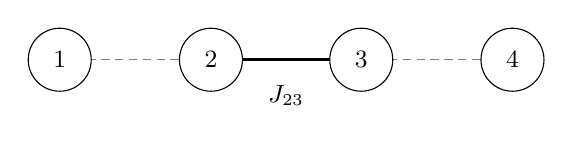
\begin{tikzpicture}[x=1.15cm,
   every node/.style={font=\small}]
  \draw[densely dashed,gray] (0,0)--(1.67,0);
  \draw[very thick] (1.67,0)--(3.33,0);
  \draw[densely dashed,gray] (3.33,0)--(5,0);
  \foreach \x/\lab in {0/1,1.67/2,3.33/3,5/4} {
   \node[draw,circle,fill=white,minimum size=8mm,inner sep=0pt]
     at (\x,0) {$\lab$};
  }
  \node[below] at (2.5,-0.2) {$J_{23}$};
 \end{tikzpicture}
 \caption{A four-dot exchange chain. The thick \(J_{23}\) link
 is selected for a gate on spins 2 and 3; the dashed links are
 available but intended to have small exchange during this pulse.
 Dots 1 and 3 have no direct exchange edge.}
 \label{fig:processor-four-dot-exchange}
 \label{fig:platform-exchange-selection}
\end{figure}
\FloatBarrier

The same chain shows when two pair gates can be independent during
one interval. Selecting $(1,2)$ and $(3,4)$ assigns each spin to
only one pair. If the coupling between the pairs is negligible,
their evolution factorizes:
\begin{equation}
 U_{12,34}=U_{12}\otimes U_{34}.
 \label{eq:platform-parallel-exchange}
\end{equation}
Selecting $(1,2)$ and $(2,3)$ instead makes spin 2 participate in
both interactions, generating a three-spin evolution that must be
designed as such. Exchange gates on edges with no shared spin are
therefore candidates for one parallel layer, provided unselected
couplings and spectator responses are also controlled.
Appendix~\ref{sec:processor-parallel-exchange} develops the resulting
scheduling conditions.

The physical exchange graph describes couplings between spins.
Its edges have different logical meanings for different encodings:
an internal edge of a three-spin block rotates one exchange-only
qubit, whereas an edge between blocks participates in a two-qubit
sequence. For two singlet--triplet blocks,
Eq.~\eqref{eq:st-capacitive-coupling} contributes a $Z_AZ_B$
interaction whenever $\kappa$ is nonzero, including during local
rotations. The same voltages can change both the local Hamiltonians
and $\kappa$. Independent logical gates therefore require the
unwanted interaction to be suppressed or refocused; otherwise the
full coupled evolution must be used. Appendix~\ref{sec:calibration-parallel-st-gates}
works through this control constraint.

\subsection{Acting on qubits without a direct link}

The four-dot graph has no exchange edge between sites 1 and 3.
One way to act on the states at those sites is to use a SWAP to
bring them onto an available edge. If $S_{23}$ exchanges the
states at sites 2 and 3 and $U_{12}$ is the desired operation
available on edge $(1,2)$, then
\begin{equation}
 U_{13}=S_{23}U_{12}S_{23}.
 \label{eq:platform-routed-gate}
\end{equation}
The rightmost SWAP brings the original state of site 3 to site 2,
and the leftmost restores the placement after the gate. This
identity holds for unknown or entangled inputs, because SWAP
permutes states without measuring them. Each dot remains occupied.
For an encoded qubit, swapping a single constituent spin generally
does not exchange the complete logical state; its logical
permutation must be constructed separately.
Appendix~\ref{sec:processor-swap-routing} develops SWAP routing
and the operations required along a longer path.

Shuttling provides another route by moving the electron itself
between dots. The transfer must avoid unwanted charge excitation
and spin flips, and the phase accumulated in the changing local
field must remain known or reproducible. The measured interdot
coupling and voltage-to-detuning response constrain the allowed
plunger-ramp speed, and the measured spin
phase sets the correction after transfer
(Appendix~\ref{sec:processor-shuttling}).
A shared quantum mode
can instead mediate an interaction while the electrons remain in
place; the useful interaction must compete with spin decoherence
and loss from the mode. The measured spin--mode couplings and loss
rates determine the usable detuning and interaction time
(Appendix~\ref{sec:processor-mode-coupling}).

The controls and detectors must also distinguish the intended
objects in an array. The measured voltage responses of the target
and affected neighbours determine the compensating electrode
changes needed to preserve their required energies and couplings
(Appendix~\ref{sec:processor-array-compensation}).
When several spins are read out, their converted charge
records must be distinguishable through the available sensors or
through measurements separated in time. Mean charge signals alone
do not specify joint outcome probabilities; correlations require
retaining the associated outcomes from each repetition.
Appendix~\ref{sec:processor-array-readout} develops the conditions
for separating those signals.
